

%\section{Introduction}
%{\color{Fuchsia}After presenting \prototype{}, the instance of our framework \framework{} meant to explore visually data warehouses, we dedicate this chapter to discuss other instances of our framework \framework{} that permit the visual exploration of other sorts of data.
%
%More precisely, we discuss first in Section~\ref{sec:bruder} a solution for visual exploration of large dynamic graphs. Subsequently, we discuss in Section~\ref{sec:prov-structu-summary} a second instance of our framework \framework{} that offers visual exploration of provenance data. 
%
%It is worth stressing that these two instances implement so far partially our framework \framework{}. To this end, we limit our discussion to the description of the new approaches proposed so far for the two instances to implement modules present in the architecture of our framework \framework{} (cf.~Figure~\ref{fig:archi-FW}).
%
%Finally, we point out that the content of this chapter relies mainly on approaches and techniques discussed in~\cite{Bruder2019,Houssem:19:TaPP}.
%}
%
%
%
%\section{Volume-based large dynamic graph analysis}
%\label{sec:bruder}
%


{\color{Fuchsia}We dedicate this section to discuss the instance of our framework \framework{} meant to the visual exploration of dynamic graphs. 
We note that this instance implements so far the \emph{provenance engine module} of our framework.
Therefore, we give a special attention to the provenance capture methodology supported so far in this instance of our framework. }



\subsection{Overview of large dynamic graph exploration}\label{A02:overview}
The volume-based large dynamic graph analysis solution is an instance of our visual data exploration framework \framework{}.
It is based on a volume-based approach proposed in~\cite{Bruder2019} where we propose methods to allow for interactive analysis of dynamic graphs containing several thousand time steps and hundreds of nodes.
	
\begin{figure}[b]
	\centering
	\includegraphics[scale=0.3]{figures/evoDM/stacking-crop}
	\caption{Sample of explored adjacency matrices~\cite{Bruder2019}}
	\label{fig:illu}
\end{figure}

Inspired by space-time cube approaches (e.g.,~\cite{bach:2017} and~\cite{Bach_CHI:14}), this instance of our framework adopts a volumetric representation of the dynamic graph.
This particular representation is illustrated in Figure~\ref{fig:illu}.
More specifically, to construct a volumetric representation of the dynamic graph, individual time steps of the dynamic graph are initially represented as adjacency matrices.
Those latter are stacked into space-time cubes.
This results in three dimensional volume structure where the $x$- and $y$-axes represent nodes, while entries in the plane defined by those two axes represent edges (including their weights). 
The $z$-axis represents time.
{\color{Fuchsia}Overall, this kind of visualization corresponds to the \emph{data display} sub-module present in the architecture of our framework as shown in Figure~\ref{fig:archi-FW}.}



To allow for fluent user interactions, the instance of our framework~\cite{Bruder2019} offers a set of analytic methods, used to explore large dynamic graphs. {\color{Fuchsia}These methods present the implementation of the \emph{data retrieval} module present in the architecture of our framework as depicted in Figure~\ref{fig:archi-FW}.}
Essentially, we distinguish the following three classes of analytic methods.
% {\color{Fuchsia}(equivalent to exploration queries in our framework)}.

\begin{description}
	\item[Data Views.] 
A single visualization is often not capable to convey all information of the exhibited large dynamic graphs.
Therefore, several data views are proposed to visualize large dynamic graphs.
This includes for instance the volume view, the timeline plot and slice views that are detailed in~\cite{Bruder2019}.
	\item[Aggregation and Filtering.] 
Filtering and aggregation of adjacent edges an essential part of the analysis process to reduce the visualization of large dynamic graphs to relevant information.
Examples of aggregation functions include for instance minimum, maximum, average weight and density of edges. These methods could be applied either on in the spacial domain i.e. aggregating neighboring edges or in the time domain.
Filtering methods consists of omitting edges not satisfying such predicate, e.g., filter out edges with low density.
\item[Comparison.] 
Comparing different sections within a temporal graph or even several distinct dynamic graphs is supported via the comparison function. 
In this case, a matrix view is generated to render commonality and irregularities resulting from comparing the different time sequences or distinct dynamic graphs.
\end{description}

		
\subsection{Evolution provenance model}
\label{A02:evoDM}
{\color{Fuchsia}In what follows, we discuss the implementation of \emph{provenance engine} module present in the architecture of our framework as shown in Figure~\ref{fig:archi-FW}.
Recall that this module is responsible of capturing provenance in the course of the visual data exploration process. Accordingly, we discuss the provenance data model adopted to track visual exploration of large dynamic graphs.
%In this case, evolution provenance keeps track of the set of visual analysis steps performed and thereby construct the ``full story'' of a visual analysis session.
%For that, we have implemented our evolution provenance model presented in Section~\ref{subsec:evo} to track the visual analytics process of large dynamic graphs. 
To do that, we define necessary analogous concepts necessary to define the evolution provenance.}

Using our volume-based large dynamic graph analysis instance~\cite{Bruder2019},
users are engaged in a \emph{visual analysis session} where they perform various \emph{visual analysis steps} iteratively.  In this context we define a  \emph{visual analysis step}  as follows.

\begin{definition}[Visual analysis step] 
Given an initial dynamic graph $G_i$ that contains a set of timesteps $\{t_1..t_i\}$, we define a visual analysis step as $\exploreStep$ where a dynamic graph $G_s$  that contains $\{t_i..t_j\}$ timesteps  (where $1 \leq i \leq j \leq k $) is visualized using a set of views $V_s=\{v_1..v_p\}$.
\end{definition}


Notice that view is a generic term that covers visualization structures possibly obtained using \emph{data views} analytic method.
In our current implementation, the evolution provenance collector tracks visual analysis steps encompassing the volumetric representation as our main view.
For future work, we also plan to integrate tracking of slice views and the timeline plot.

%\begin{table}[t]
%\taburowcolors[2]{white .. black!10}
%\sffamily\footnotesize
%\tabulinesep=4pt
%\begin{tabu}{|X[cm]|X[cm]|X[cm]|}
%\hline
%\rowcolor{black!80} \color{white}Operation type &   \color{white}Parameters& \color{white}Output\\
%Selection&  $\{t_{i'}..t_{j'}\}$; selected range of timesteps & $G'_{s}=\{t_{i'}..t_{j'}\}$,  $V'_{s}=\{v'_{1}..v'_{p}\}$\\
%Partition&$\{m_1..m_y\}$; the set of split marks & $G'_{s}=[\{t_1..t_m\},\{t_{m+1}..t_l\},..]$ ,  $V'_{s}=\{v'_{1}..v'_{p}\}$ \\
%Aggregation&    $l$, where $l$ is a level & $G_{s}$,  $V'_{s}=\{v'_{1}..v'_{p}\}$ \\
%Filtering&    $cond$, where $cond$ is a predicate& $G_{s}$,  $V'_{s}=\{v'_{1}..v'_{p}\}$ \\
%Color mapping&  $d \times rgb $, where $rgb$ is color and $d$ a graph property &$G_{s}$,  $V'_{s}=\{v'_{1}..v'_{p}\}$ \\
%Camera configuration&  $configuration$   & $G_{s}$, $V'_{s}=\{v'_{1}..v'_{p}\}$ \\
%\hline
%\end{tabu}
%\caption{Permitted analytics operations~\cite{Bruder2019}}
%\label{table:ops}
%\end{table}



\begin{table}[b]
 \centering \scriptsize
 \begin{tabular}{|p{2.5cm}|p{4cm}|p{3cm}|} \hline
\textbf{Operation type}  & \textbf{Parameters} & \textbf{Output}  \\ \hline
Selection&  $\{t_{i'}..t_{j'}\}$; selected range of timesteps & $G'_{s}=\{t_{i'}..t_{j'}\}$,  $V'_{s}=\{v'_{1}..v'_{p}\}$ \\ \hline
Partition&$\{m_1..m_y\}$; the set of split marks & $G'_{s}=[\{t_1..t_m\},\{t_{m+1}..t_l\},..]$ ,  $V'_{s}=\{v'_{1}..v'_{p}\}$  \\ \hline
Aggregation&    $l$, where $l$ is a level & $G_{s}$,  $V'_{s}=\{v'_{1}..v'_{p}\}$ \\ \hline
Filtering&    $cond$, where $cond$ is a predicate& $G_{s}$,  $V'_{s}=\{v'_{1}..v'_{p}\}$  \\ \hline
Color mapping&  $d \times rgb $, where $rgb$ is color and $d$ a graph property &$G_{s}$,  $V'_{s}=\{v'_{1}..v'_{p}\}$  \\ \hline
Camera configuration&  $configuration$   & $G_{s}$, $V'_{s}=\{v'_{1}..v'_{p}\}$  \\ \hline
\end{tabular}
\caption{Permitted analytics operations~\cite{Bruder2019}}
\label{table:ops}
 \end{table}

Table~\ref{table:ops} summarizes supported analytical operations enabling the navigation from a visual analysis step $\exploreStep$ to another step $\exploreStepDest$.
It presents also the set of parameters needed for each operation as well as the structure of the output analysis step $S'$.
Essentially, we distinguish six operation types that handle various views seen over several analysis steps.
All proposed operations to track in evolution provenance are derived from the three fundamental analytic methods thoroughly discussed in Section~\ref{A02:overview} that are data views, filtering/aggregation and comparison.


The \emph{selection function} is associated to the timeline plot feature where the user gets a 2D-visualization whose x-axis depicts a set of timesteps $\{t_i..t_j\}$.
Using this function, the user can select a single or a range of timesteps $\{t_{i'}..t_{j'}\}$  with $t_i \leq t_{i'} \leq t_{j'} \leq t_{j}$ to analyze them visually in the next step.

The \emph{partition operation} corresponds to the volume partitioning analysis feature 
where the user specifies interactively some split marks $\{m_1..m_y\}$ to split the timesteps $\{t_1..t_i\}$ associated to a visual analysis step $S$ into sub-ranges $[\{t_1..t_m\},\{t_{m+1}..t_l\},\ldots]$. 


The evolution provenance model implemented for the volume-based large dynamic graph analysis solution encompasses also the \emph{aggregation operation} and the \emph{filtering operation} (via opacity). 
The former aggregates to a specific level $l$ to alleviate the complexity of a view $V$, while the latter operation omits information available in the current view that do not satisfy a predicate $cond$. As shown in Table~\ref{table:ops}, the two aforementioned operations introduce changes only on the set of views to analyze in the step $S'$ in comparison to step $S$ while keeping the same dynamic graph $G_s$.

The list of analytics operations recorded by our provenance model also contains the \emph{color mapping operation} where a user maps a graph property $d$ (e.g., weights of edges) to a specific range of colors $rgb$ to produce new views $V'_{s}=\{v_{i'}..v_{j'}\}$ for the same dynamic graph $G_s$, seen in the analysis step $S$. 
Finally, we record selected \emph{camera configurations}, where the user selects a certain zoom level, rotation and panning of the camera to get new views $V'_s$ in the next analysis step $S'$.

Overall, the evolution provenance captured by this particular instance of our framework \framework{} is modelled by an analysis session graph that gathers all visual analysis steps made by the analyst. 
This graph is defined as follows.

%\begin{figure}[t]
%	\begin{center}
%	\includegraphics[scale=0.35]{figures/evoDM/sessionGraph-crop}
%			\end{center}
%			\caption{Example of an analysis session graph, augmented with images of the respective analytics steps~\cite{Bruder2019}}
%			\label{fig:expo-session}
%\end{figure}

\begin{definition}[Analysis session graph]
An analysis session graph summarizes user's manipulations over a large Dynamic Graph $D_i$ where $i$ refers to the set of timesteps.
The analysis session graph is a labeled directed acyclic graph (DAG) $\sessionGraph{}_{D_i}(\sessionV{}, \sessionE{})$ where $\sessionV{}$ is a set of nodes and $\sessionE{}$ a set of labeled edges. 
Each node $n \in \sessionV$ corresponds to a visual analytics step $S$.
An edge $e = (n, n', \sessionL{})$ represents the transition from one visual analytics step $S = \{{G_s}, V_s\}$ to the next visual analytics step $S' = \{{G'_s}, V'_s\}$. $\sessionL{}$ is a pair $\langle \labelOp{}, param \rangle$ where $\labelOp{}$ is an identifier of the analytical operation type (see Table~\ref{table:ops}) and $param$ is the set of parameters used to navigate from $S$ to $S'$.
\label{def:sessionA02}
\end{definition}


%%{\color{Fuchsia}Overall, the evolution provenance is implemented in the volume-based large dynamic graph analysis solution~\cite{Bruder2019} following our proposed data model specified in Definition~\ref{def:session}.
%%Accordingly, 
%{\color{Fuchsia}Overall, the evolution provenance of the volume-based large dynamic graph analysis instance~\cite{Bruder2019} is a graph that gathers all visual analysis steps (analogous to exploration steps) made by the analyst. 

Figure~\ref{fig:expo-session} shows an example of such an analysis session graph (augmented with exemplary screenshots of the analytics step).

\begin{figure}[b]
	\center
	\includegraphics[scale=0.35]{figures/evoDM/sessionGraph-crop}
			\caption{Example of an analysis session graph, augmented with images of the respective analytics steps~\cite{Bruder2019}}
			\label{fig:expo-session}
\end{figure}

Essentially, {\color{Fuchsia}nodes of the analysis session graph (evolution provenance)} correspond to the set of visual analytics steps and edges represents the transition from one visual analytics step to another. %visual analytics step. 
Note that, the labels of edges contain so far only type of navigation and set of parameters used to navigate. In the future, we intend to implement the score $s(e)$ (specified in Definition~\ref{def:session}) that reflects the importance of each edge present in the analysis session graph.


{\color{Fuchsia}We have described in this section the instance of our framework \framework{} meant to visual exploration of dynamic graphs. We focused mainly on the implementation of provenance capture in this particular instance. In the future, we intend to propose new approaches meant to implement the \emph{recommendation engine} module present in the architecture of our framework to provide users with a holistic recommendation-based visual exploration of large dynamic graphs. }

%
%
%\section{Visual analytics of provenance summary}
%\label{sec:prov-structu-summary}
%
%%\subsection{Introduction}
%%\label{sec:intro}
%
%As we have shown in Section~\ref{sec:prov-type}, various systems and approaches have been proposed to collect different types of provenance for various use cases, e.g., for the reproducibility and the debugging of complex computational processes~\cite{Herschel2017survey}. Therefore, the visual exploration of provenance allows users to get a better understanding of results and may lead to the discovery of information helpful to refine the computational processes for which provenance is tracked.
%{\color{Fuchsia}In this context, we propose in this chapter a new approach that summarizes many provenance traces conforming the PROV-JSON\footnote{\url{https://www.w3.org/Submission/2013/SUBM-prov-json-20130424/}} standard. We further describe the analysis tasks that apply on these summaries. 
%Note that we use in this chapter the term \emph{provenance trace}  to refer to a single provenance graph collected in one run of the computational processes for which provenance is tracked.}
%To clarify our contribution, let us consider the following example. 


In the previous chapters, we have described our provenance-based framework that provides a holistic approach to support users in exploring data visually.
 Part of our proposed solution are evolution provenance graphs that represent either individual user exploration sessions or summaries of multiple user sessions. During our research, we noticed the value of analyzing these graphs, especially the summary graph. One very simple example is the discussion in Section~\ref{collaborative-query-rec}, where analyzing the topology of evolution provenance summary graph helped us to gain further insights on global trends commonly opted by users when exploring visually data.
To better support such analysis, we present in this chapter a general approach meant to summarize various types of provenance conforming the standard exchangeable format for provenance PROV-JSON\footnote{\url{https://www.w3.org/Submission/2013/SUBM-prov-json-20130424/}}. We further describe the analysis tasks that apply to these summaries. 
Note that we use in this chapter the term \emph{provenance trace} to refer to a single provenance graph collected in one run of the computational processes for which provenance is tracked.
To clarify our contribution, let us consider the following example. 



\begin{figure}[b]
\includegraphics[scale=0.4]{figures/tapp19/example_traceMIT.pdf}
\caption{Excerpt of evolution provenance collected in \prototype{}}
\label{fig:universityX}
\end{figure}


\begin{example}
  \label{par:example}
We performed a user study to examine methodologies and practices adopted when exploring data visually.
To do that, we hired ten students and we asked them to explore various data warehouses using \prototype{}, the instance of our framework \framework{}.
 To better understand the behaviour of users during the user study, we have collected the evolution provenance tracking explorations made by each participant. 
 These evolution provenance graphs are converted to the PROV-JSON, a standard, exchangeable format. 
 Figure~\ref{fig:universityX} depicts an excerpt of the evolution provenance (comprising around 100 edges/nodes) tracked from one exploration session made in the user study. This provenance trace conforms to the PROV-JSON format. 
 Essentially, ``agent1'' corresponds to the user performing this exploration session. We have also in this excerpt of evolution provenance trace three manipulations that are represented in Figure~\ref{fig:universityX} as three activities:  ``activity0'', ``activity1'', and ``activity2''.
``activity0'' corresponds to the initial SQL query specified by the user in \prototype{} to start an exploration session. ``activity1'' refers to the computation of recommendations in the course of the exploration while ``activity2'' corresponds to the user's request to investigate the Zoom-In recommended query (cf.~Example~\ref{ex:query-ZoomIn}) associated to attribute $a1$.
 Those activities are associated with the user ( see edges with labels ``assoc'').
 These activities are involved in the generation of three entities: ``entity0'', ``entity1'', and ``entity2''. 
 The two entities  ``entity0'', and ``entity1'' correspond to the exploration steps while the entity ``entity2'' refers to an impact matrix containing scored recommendations (cf.~Example~\ref{ex:sampleMatrix}).
 \end{example}
%  {\color{Fuchsia}Actually, the excerpt of evolution provenance trace shown in Figure~\ref{fig:universityX} is part of a large graph that contains an important number (around hundred) of vertices and edges. Accordingly, the visualization of the full evolution provenance trace associated {\color{Fuchsia}to one exploration session} is a cumbersome task. This complicates thereby the process of understanding users' behaviour when exploring visually the set of  evolution provenance traces captured in the course of the user study.}
%Furthermore,  the analysis of a single evolution provenance trace alone is not sufficient to understand the global users' behaviour in the course of the user study. Yet, in this example, it would be more interesting to find out how this evolution provenance trace relates to provenance traces of other participants. This calls for generating evolution provenance traces for the ten participants and comparing those.  However, visually comparing all evolution provenance traces quickly becomes infeasible.
%\mel{ the generalization to overall summarization for a given purpose should be spelled out (this is somewhat your problem statement, i.e., how to summarize graphs such that ...).}
%\end{example}
As mentioned in the example, we aim at studying users' behavior when exploring data using \prototype{}.
Hence, it would be interesting to find out how evolution provenance traces of participants relate to each other. 
Yet, a simple evolution provenance graph easily reaches a large size. 
Consequently, comparing all evolution provenance traces quickly becomes infeasible.




To simplify the comparative task motivated above, we propose in this chapter our structural-based summary approach.
Our proposed approach infers initially the general structure of each provenance trace. The individual structures are then unified in a merged structure with annotations that quantify the coverages of sub-structures in the underlying collection of provenance traces. In what follows, a particular attention is given to the explanation of our proposed summary approach.

\begin{figure}[b]
\includegraphics[scale=0.4]{figures/tapp19/example_trace_summary.pdf}
\caption{Structural summary of ten evolution provenance traces}
\label{fig:Inf-type-university}
\end{figure}

\begin{example}\label{par:example2}
 The structural summary of the ten evolution provenance traces collected in the course of our user study is depicted in Figure~\ref{fig:Inf-type-university}. Vertices present different structures available in the ten provenance traces. 
 We distinguish mainly three families of structures: (i) entities structures: they are depicted as yellow circles in Figure~\ref{fig:Inf-type-university} (ii) activities structures: they are depicted as blue boxes in Figure~\ref{fig:Inf-type-university} and they present structures inferred from activities present in Figure~\ref{fig:universityX} and (iii) agents structures: they are depicted in orange trapezoid in Figure~\ref{fig:Inf-type-university} and they are inferred from agents present in Figure~\ref{fig:universityX}. 
 Each structure definition is depicted in a white box near each vertex. Each edge is associated with two annotations that specify the type of provenance relationship and its frequency in the analyzed provenance traces. 
 From this graph, we see that the activity structure ``actST5'' was the most present among available structures of activity. Recall that  the structure ``actST5'' corresponds to the situation where the user is asking for recommendation to explore interesting regions of the data.   This indicates that users rely mainly on recommendations suggested alongside the visual data exploration process.
 Based on the edge linking the structure  ``actST5'' and the structure ``entSt1'', we see that 90 recommendation sets were proposed to the ten participants in the user study.   Among the 90 set of recommendations, we see that users prefer mostly to investigate recommendations of type `` Zoom-In'' (see the cardinality of edge linking ``actSt1'' and ``entST0''). Contrarily, a low number of recommendations of type extension were investigated by the participants in the user study (the cardinality of the edge between ``actSt4'' and ``entST0'' is equal to 25).
 
From this summary, we can learn some common practices adopted by users when exploring data visually using \prototype{}.
For instance, it becomes clear that we can distinguish types of recommendations commonly opted (e.g. recommendations of type ``Zoom-In'') from those less solicited by users (e.g., recommendations of type ``Extension'') when exploring data using \prototype{}.
\end{example}





The example above provides one motivating scenario that demonstrates the usefulness of the structural provenance summary approach.
Further use cases are discussed in Section~\ref{sec:casestudy}. To achieve the functionality described in the example, we propose an end-to-end solution that infers the schema of multiple provenance traces in W3C-PROV format  to then summarize those in one graph. 
This approach has several benefits including (i)~the summary allows to get a first rough overview about a collection of provenance traces; (ii)~it is useful to highlight commonalities and differences among the traces for comparative analysis, and (iii)~it allows to pinpoint corner cases and exceptions. 



Overall, our proposed approach ensures the following contributions.
\begin{itemize}
\item \textbf{Provenance structure summarization}. We propose a two-phase algorithm to produce the structural summary of provenance traces. The first step infers the structure of each individual trace. These structures are then input to the second phase that produces the merged and weighted provenance structure summary graph, where weights translate the coverage of a relationship in the individual traces. %\mel{shouldn't the coverage be sth between 0 and 1?}
\item \textbf{Provenance summary visualization and analysis.} We define several visual analysis tasks over the summary graph. For selected tasks, we showcase different visualizations as part of our preliminary use-case based evaluation.%  for 
\item \textbf{System implementation and evaluation.} We implement the proposed approach in a prototype, for which we provide a preliminary performance evaluation. Results show the effectiveness of our approach in terms of runtime and conciseness of inferred summaries. %structures-based summaries.
\end{itemize}

The remainder of this section is structured as follows. Section~\ref{sec:related} discusses related work. Section~\ref{sec:prelim} covers necessary definitions and formal preliminaries. We present our structure-based summary approach in Section~\ref{sec:system}. Visual analysis tasks and use cases are presented in Section~\ref{sec:vis} and Section~\ref{sec:casestudy}. Finally, we discuss our implementation and evaluation in Section~\ref{sec:evaluation}. 
Note that the content of this section is mainly based on methods and approaches described in~\cite{Houssem:19:TaPP}, which are based on our early work~\cite{baazizi2017}.
%\subsection{Related work}
%\label{sec:related}
%This section reviews research in fields related to our work, i.e., provenance summary and schema inference and integration.
\subsection{Summary of provenance traces}
Several strategies have been proposed to simplify a single provenance trace.
One of them is the temporal-based strategy which was widely adopted by many works including~\cite{Bork13,Stitz:2016}. 
%\mel{how it is working? briefly}
This strategy consists of clustering provenance information that was tracked in the same time frame. While this strategy reduces successfully the complexity when dealing with one provenance trace, it does not apply on a set of provenance traces collected at different periods.

Other strategies include semantic summaries~\cite{Ainy:2015,OliveiraMOOB16,KoopFS13}.
These require expert knowledge to define semantic mappings between provenance components. The same holds for the user-defined summaries~\cite{MissierBGCD14,Biton:2007}, where sufficient user knowledge about the processed provenance trace is required to appropriately perform grouping operations.

Template-based summarization consists in merging sub-parts of an analyzed provenance trace when they have the same shape (template)~\cite{Stitz:2016}. However, the specification of these templates is left to users, i.e., they have to specify patterns they expect in their provenance traces that can be collapsed in a simplified visualization.
In the same context, Moreau et al.~\cite{Moreau15} propose a parametric summary solution that compresses firstly paths of size $k$ and then merges compressed paths having the same shapes. While this solution could be applied on a set of provenance traces, it is still unclear how to set a reasonable value of $k$ that generates a concise summary neither too general nor too specific.




Finally, approaches such as~\cite{Moreau18,Curcin:2017} declare a template subsequently collected provenance follows. This template can be seen as a static summary that is independent of the set of analyzed provenance traces. 
Opposed to generating a static summary, our approach considers actual provenance traces and exposes their similarities and differences. Our approach reveals also which parts of the static summary are actually covered by the set of analyzed provenance traces. 




%Overall, our work differs from discussed works in two main aspects: (i)~most of the discussed works rely on expert knowledge to summarize provenance. This is not required using our approach; (ii)~opposed to approaches generating provenance templates using a top-down approach, we follow a bottom-up strategy to infer structures from analyzed provenance traces.

\subsection{Schema inference and schema integration}
Our approach is close in spirit to schema inference, where given a set of datasets, a common, generalized schema in a predefined data model is derived. Given our focus on semi-structured W3C PROV provenance traces, our work is closely related to schema inference for XML and JSON data~\cite{hegewald:icdews06,baazizi2017}.

Our work is also related to schema integration, especially for semi-structured data~\cite{chiticariu:sigmod08}  where, given a set of schemas, a unified schema is determined. This latter covers all concepts and properties of the input schemas and correctly models the constraints defined in these input schemas.  

While the above methods may complement our approach, they are left for future research. In particular, integrating such techniques requires to further investigate the information loss and associated impact on analytical applications on provenance traces.
Our current focus lies on inferring a structural summary that reports primitive types of provenance components and that highlights dependencies (an important aspect for provenance analysis) between inferred structures. 
%\mel{not convincing}




%
%
%\subsection{Preliminaries and system overview}
%\label{sec:prelim}
%As discussed earlier, we propose a solution relying on structural aggregation for visual provenance analysis. This solution follows the pipeline shown in Figure~\ref{fig:overview}, briefly described below.  
%{\color{Fuchsia}As discussed earlier, we propose an instance of our framework \framework{} that is meant to explore provenance traces.
%Our instance leverages a novel solution structural aggregation approach to facilitate the visual exploration of provenance. This solution follows the pipeline shown in Figure~\ref{fig:overview}, briefly described below. }


\begin{figure}[b]
\centering
 \includegraphics[scale=0.4]{figures/tapp19/overview.pdf}
 \caption{Overview of the proposed approach}
 \label{fig:overview}
\end{figure}

\smallskip
\noindent \textbf{Individual W3C-PROV graphs.} We assume that all input provenance traces conform to the W3C-PROV data model~\cite{w3c-prov-dm}. 
%
As defined in~\cite{MissierBGCD14}, this data model defines three types of sets: (i)~Entities (\emph{En}), i.e., data, documents; (ii)~Activities~(\emph{Act}), i.e., processes, actions acting upon entities; and (iii)~Agents (\emph{Ag}), i.e., humans, software. The W3C-PROV data model further defines a set of relationships among entities, activities, and agents. Examples of relationships include for instance:\\
$usage:use \subseteq Act \times En$ 
\hspace{1.2cm}
$attribution:att \subseteq En \times Ag$\\
%\hspace{1cm}
$derivation:der \subseteq En \times En$
\hspace{0.5cm}
$generation:gen \subseteq En \times Act$\\
$delegation:del \subseteq Ag \times Ag$
\hspace{0.5cm}
$association:assoc \subseteq Ag \times Act$\\

\hspace{-1em}Note that the W3C-PROV data model has many variations. In what follows, we focus mainly on the PROV-JSON representation of the W3C-PROV given the wide adoption of JSON as an exchangeable data format. This allows us to reuse existing solutions, e.g., for JSON schema inference~\cite{baazizi2017} or visualization frameworks. %\mel{too vague} 
Furthermore, JSON is semi-structured and thus allows to easily model heterogeneous provenance traces. 




A PROV-JSON provenance trace follows the tree format displayed in Figure~\ref{prov-json-skeleton}. % where the provenance trace is presented as a tree.
Each information present at the top-key level maps to a W3C-PROV concept described above. 


\begin{figure}[t]
\centering
	\begin{minipage}{1\textwidth}
			\begin{center}
				\resizebox {0.9\textwidth} {!} {
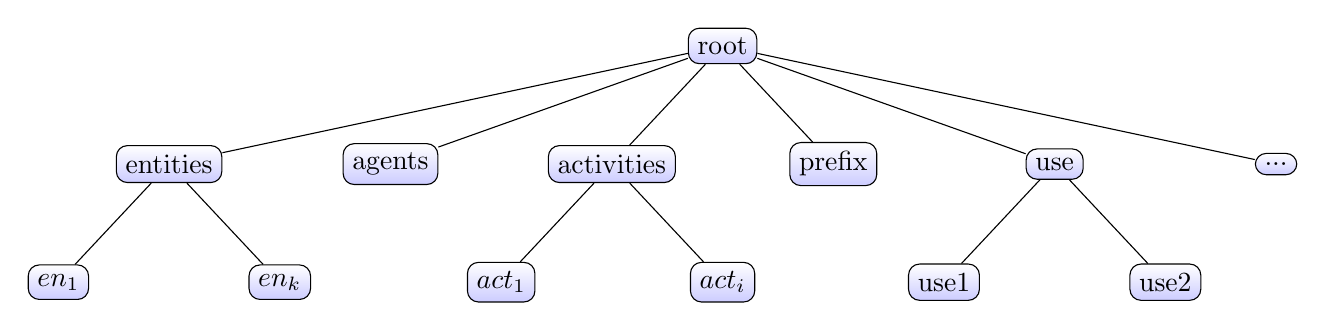
\begin{tikzpicture}[sibling distance=8em,
  every node/.style = {shape=rectangle, rounded corners,
    draw, align=center,
    top color=white, bottom color=blue!20}]]
  \node {root}
    child { node {entities}
         child { node {$en_1$} }
         child { node {$en_k$} }
     }
      child { node {agents} }
    child { node {activities}
      child { node {$act_1$} }
        child { node {$act_i$} }
        }
        child { node {prefix} }
        child { node {use}
        child { node {use1} }
        child { node {use2} }
        }
           child { node {...} }
        ;
\end{tikzpicture}
}
\end{center}
\end{minipage}
\caption{Top-key level of a PROV-JSON trace}
\label{prov-json-skeleton}
\end{figure}



The provenance traces represented in PROV-JSON format generally form a graph, that we define as follows. 

\begin{definition}[Provenance graph]
\label{def:prov-graph}
A provenance graph is a directed graph $G_P(V, R)$, where $V$ is the set of vertices and $R$ maps to provenance relationships.
Let $root \subseteq V$ be a set of vertices with an in-degree of 0 and an out-degree larger than 0. These nodes represent entities that are derived as described by the provenance trace. Successors of $root$ are entities $En \subseteq V$, activities $Act \subseteq V$, and agents $Ag \subseteq V$ involved in generating the entities described by $root$.
Each edge $e = (\langle v_{1},v_{2} \rangle,t)$, represents a provenance relation $r \subseteq R$ of type $t$ (e.g. gen, use) between $v_{1}$ and $v_{2}$  where   $\{v_{1},v_{2}\} \subseteq V$.
\end{definition}


    Figure~\ref{fig:universityX} depicts an example of a provenance graph.
     %obtained  {\color{Fuchsia} when exploring data warehouses using \prototype{}, the instance of our visual data exploration framework \framework{}.
%    It describes the why-provenance of the result ranking of ``MIT'', that is, it returns the source data relevant to produce this result.
%    The set  $root$ contains a unique entity ``entity1'' that results from the ranking query.
%    This latter is presented as an activity that uses the entity ``entity0'' to generate the result. 
%    Figure~\ref{fig:universityX} further includes white boxes associated with each node in the provenance graph. These contain the concrete provenance information recorded for each node. For instance, the provenance recorded about ``entity1'' includes the name of the university and the ranking value.
    It describes the set of explorations steps (cf.~Definition~\ref{def:expo-step}, Page~\pageref{def:expo-step}) investigated  by the user. The set  $root$ contains the entity ``entity2'' (corresponding to the last reached exploration step )  and  the agent ``agent1'' (corresponding to the user). Figure~\ref{fig:universityX} further includes white boxes associated with each node in the provenance graph. These contain the concrete provenance information recorded for each node. For instance, the provenance recorded about ``entity2'' includes the ids of the query and the visualization inspected by the users.

\smallskip


\noindent \textbf{Structure-based provenance summarization. } The set of provenance graphs defined above serve as input to our structure-based provenance summary approach, which consists of two steps. First, we infer individual provenance structures associated to individual provenance traces (local structures inference in Figure~\ref{fig:overview}). The second step aggregates individual structures into a single W3C-PROV compliant graph that structurally summarizes input provenance traces. 
More formally, we define the structure-based summary graph as follows.


\begin{definition}[Structure-based summary graph]A structure-based summary graph is a W3C-PROV compliant directed graph $SSG(PS_s, RS_s)$ associated to a set of provenance graphs $G$=\{$G_{P1}, \ldots,G_{Pn}$\} where $PS_s$ is the set of vertices referring to provenance structures defined later in Definition~\ref{def:prov-type} and $RS_s$ are edges mapping to the set of inferred provenance relationships. %\mel{Re reviewer 1: maybe ref to inference rules?)} 
Each relation $r \subseteq RS_s$ is presented as $ (\langle ps_{1},ps_{2}\rangle,t,c)$ where  $\langle ps_{1},ps_{2}\rangle$ is the edge connecting two structures $ps_1, ps_2 \in PS_s$, the type $t$ presents the provenance relationship type, and the cardinality $c$ is the number of provenance relationships in $G$, that follow the structure of $r$.
%quantifies the coverage of $r$ in $G$. 
\end{definition}


Figure~\ref{fig:Inf-type-university} shows an example of a structure-based summary graph. % inferred using our approach from provenance traces discussed in our illustrative Example~\ref{par:example}.
The content of this graph is discussed in Example~\ref{par:example2}.





\noindent \textbf{Visualization and analysis.} %To support users for different kinds of analysis over the structure-based summary graph, the last component of our pipeline provides different visualizations thereof.
The last component of our pipeline generates visualizations suited for various visual analysis tasks that rely on the structure-based summary graph. 
%{\color{Fuchsia}In contrast to previous steps depicted in Figure~\ref{fig:overview} that implement the \emph{provenance engine} module of our framework \framework{},  the visualization and analysis step describes possible techniques that can be used to implement the \emph{data display} module present also in the architecture of our framework \framework{} (cf.~Figure~\ref{fig:archi-FW}).}



\smallskip
%After this overview of the individual components of our solution, we now delve into the details of the structure-based provenance summarization component (Figure~\ref{sec:system}) and the visualization component (Figure~\ref{sec:vis}).
After this overview, we now delve into the details of individual components of our solution in Section~\ref{sec:system} and Section~\ref{sec:vis}.


%
%
%\subsection{Provenance structure inference}
%\label{sec:system}
%\begin{figure}[b]
\[  \scalemath{0.8}{
\begin{array}{lllllll}
p ::=  Act \mid En \mid Ag  & \text{provenance high level types} \\
Act,En,Ag ::=  \epsilon \mid R  & \text{provenance types} \\
R ::=	\{ l_1:s_1, \ldots, l_i:s_i \}    & \text{Record type} \\
s::=    R \mid A \mid Bs  & \text{structure types} \\
A ::=  [s_1, \ldots,s_j]&\text{Array type} \\
B ::=	 \nule \mid Bool \mid \ Num \  \mid \ Str  & \text{Basic type}\\
\end{array} }
\]
 \vspace{-1.5em}
\caption{Syntax of provenance types}
\label{fig:datamodel}
\end{figure}





Figure~\ref{prov-json-skeleton} shows the top-key level structure of a PROV-JSON provenance trace, which contains nodes referring to W3C-PROV relationships (e.g., use, gen). Those nodes have always standard structures respecting the constraints defined in the W3C-PROV data model. In contrast, nodes mapping to entities, activities, and agents may have various structures (e.g., entities ``entity0'' and ``entity1'' in Figure~\ref{fig:universityX}) depending  on the underlying provenance collector.
Hence, a special focus is given in what follows to the subset of top-key level's elements, called provenance components, that contains entities, activities, and agents.
The provenance components follow the syntax shown in Figure~\ref{fig:datamodel}, extending the syntax proposed in~\cite{baazizi2017} to fit the content of W3C-JSON provenance traces. 



A provenance component $p$ is either an activity ($Act$), entity ($En$) or agent ($Ag$) type. 
These provenance high level types encompass records that are sets of pairs. Each pair has a label $l_i$ associated with a structure type $s$.
This latter could be a record, an array, or a basic type.
The array type is a sequence of structure types $s$ while basic values $B$ comprise $null$ values, booleans $Bool$, numbers $Num$, and strings $Str$.





%\subsection{Prov-type inference}
\subsection{Provenance component type inference}
The first phase of our approach performs a type inference for each provenance component $p$ present in the provenance trace. We adjust the inference rules proposed in~\cite{baazizi2017} to infer types called in what follows \emph{prov-types} defined in Figure~\ref{fig:datamodel}.

Prov-type inference is done according to the inference rules in Figure~\ref{fig:typinf}.
We distinguish two types of inference rules: (i)~those without premise: they infer the prov-type of value by simply reflecting the type of the value itself and (ii)~rules with premise: they require the recursive prov-type inference of each element present in the premise to generate the global prov-type indicated in the conclusion part. 



 \begin{figure}[t]
 \centering
\scalemath{0.75}{
 \begin{tabular}{llll}
 \staterule{(\textsc{TypeEmpty})}
   {}
   {
	% \judbasee{\{ \} }{  \{\} }
	 \judbasee{\{ \} }{ \tnull }
	 }
 &
 \staterule{\small(\textsc{TypeBool})}
  {}
 {\judbasee{true/false}{\tbool}}
  \\ \\
 \staterule{(\textsc{TypeNumber})}
   {s \in Number}
   {\judbasee{s}{\tnum}}
 &
 \staterule{(\textsc{TypeString})}
   {s \in String}
   {\judbasee{s}{\tstr}}
\\ \\
 \multicolumn{1}{c}{\staterule{(\textsc{TypeArray})}
{\judbasee{s_1,\ldots s_n}{T_1,\ldots,T_n} }
{\judbasee{[s_1,\dots,s_n]}{[T_1,\dots,T_n]}} }
   &
 \multicolumn{2}{c}{\staterule{(\textsc{TypeRec})}
 {\judbasee{s_i}{T_i} \ \ \judbasee{s_j}{T_j} \ \ \forall \textsc{ }{i},{j} \textsc{ }  i\neq j \Rightarrow l_i \neq l_j
 }
 {
 \judbasee{\{\fieldd{l_1}{s_i}, \ldots, \fieldd{l_i}{s_i} \} }{ \{\fieldd{l_1}{T_i}, \ldots, \fieldd{l_i}{T_i} \} }
 }}
  \\ \\

      \multicolumn{1}{c}{\staterule{(\textsc{TypeAgent})}
 {\judbasee{s}{T} }
 {\judbasee{Ag(s)}{Agent(T)}} }
&
   \multicolumn{1}{c}{\staterule{(\textsc{TypeAct})}
 {\judbasee{s}{T} }
 {\judbasee{Act(s)}{Activity(T)}} }
   &
   \multicolumn{1}{c}{\staterule{(\textsc{TypeEntity})}
 {\judbasee{s}{T} }
 {\judbasee{En(s)}{Entity(T)}} }
 \end{tabular}
}
 \caption{\label{fig:typinf}Prov-type inference rules.}
 \end{figure}



Based on inference rules presented in Figure~\ref{fig:typinf}, we can define {\emph{prov-type}}, the first step towards generating a structural provenance summary of a collection of provenance traces.
\begin{definition}[Prov-type]
\label{def:prov-type}
A prov-type for a vertex $v$ present in $G_P(V, R)$ corresponds to the structure inferred for~$v$.
\end{definition}

\begin{example}[Example of inferred prov-types]
Following our definition, the prov-type inferred for the entity ``entity0'' shown in Figure~\ref{fig:universityX} is:
\begin{center}
\small
\begin{adjustbox}{width=0.4\columnwidth,center}
\begin{tabular}{l}
\{ ``Entity'': \\
\hspace{0.5cm}	\{ \\
\hspace{0.5cm}\hspace{0.5cm}	``exp:queryID'': Num, \\
\hspace{0.5cm}\hspace{0.5cm}	``exp:visID'': Num \\
\hspace{0.5cm}	\} \\
\}
\end{tabular}
\end{adjustbox}
\end{center}
This prov-type is inferred using the recursive \emph{TypeRec} inference rule depicted in Figure~\ref{fig:typinf}. This rule is recursive. Accordingly, we iterate over key-values pairs present in entity ``entity0'' shown in Figure~\ref{fig:universityX}. For each key-value pair, we maintain the key and we apply a basic inference rule on the value (see \emph{TypeNumber} rule depicted in Figure~\ref{fig:typinf}).  Finally, the set of key and their associated basic types are grouped and returned as a result of the recursive \emph{TypeRec} inference rule.

\end{example}

\subsection{Individual structural provenance graph}
Once we compute the prov-type of each vertex in a provenance graph, we are able to infer the individual structural provenance graph that we define as follows.
\begin{definition}[Individual structural provenance graph]
  \label{def:temp-prov}
$GS(P_s, R_s)$ is an individual structural provenance graph associated to a provenance graph $G_P(V, R)$.
It is a W3C-PROV compliant directed graph where $P_s$ is the set of prov-types for all $v \in V$ and $R_s$ is the set of inferred relationships structures: 
Each edge $e_s = (\langle ps_1, ps_2\rangle,t,c)$ is a provenance relationship structure in $R_s$ between two structures $\{ps_1, ps_2\} \subseteq P_s$. The edge $e_s$ is labeled by $t$ that refers to the type of provenance relationship and  by a cardinality $c$ computed as  $c=|R_{sim}|$ such that  $R_{sim}\subseteq R$ and  $\forall  e_r=(\langle v_1, v_2\rangle,t') \in R_{sim}$, $e_s.t=e_r.t'$ holds and  $\forall i  \in \{1,2\},  \exists j  \in \{1,2\}$ such that the prov-type of $v_{i}$ is equal to $ps_j$. 
\end{definition}


Note that the following properties hold for the individual structural provenance graph $GS(P_s, R_s)$:

\begin{lemma}[Properties of structural provenance graph]
\label{def:prop}
For a structural provenance graph $GS(P_s, R_s)$, we have
\begin{itemize}
\item  $\forall ps ,ps'  \in P_s$,   $ps \neq ps'$
\item  $\forall p_s  \in P_s  $, $  \exists$  $v \in V$  such that its prov-type is equal to $p_s$
\item  $\forall e_s=(\langle ps_1, ps_2\rangle,t,c) \in R_s, \exists e=(\langle v_1, v_2\rangle,t') \in R$  such that $e_s.t=e.t'$ and $ \forall i  \in \{1,2\}, \exists j  \in \{1,2\} $ such that the prov-type of $v_{i}$ is equal to $ps_j$.
\end{itemize}
\end{lemma}

\begin{figure}[t]
\centering
\includegraphics[scale=0.4]{figures/Tapp19/EvoPROV_provSummary}
\caption{Structural summary of MIT's ranking provenance}
\label{scheme:universityX}
\end{figure}
Figure~\ref{scheme:universityX} shows an example of individual structural provenance graph associated to the excerpt of W3C-PROV evolution provenance graph shown in Figure~\ref{fig:universityX}.  It contains 6 nodes whose prov-types are shown in white boxes below each vertex. For instance, the node ``actSt0'' has a prov-type that was inferred from the node ``Activity0'' present in Figure~\ref{fig:universityX}. 
Figure~\ref{scheme:universityX} depicts also cardinalities and types associated with each edge.
For instance, the edge between ``actSt1'' and ``agSt0'' has the type ``association'' and a cardinality equals to one.
The cardinality is explained by the provenance graph shown in Figure~\ref{fig:universityX} where we have one edge of type ``association'' between nodes ``activity1'' and ``agent1''.




To infer an individual structural provenance graph, we leverage the following two fundamental definitions.
\begin{definition}[Vertex structural equality]
    \label{lm:vert}
Given a provenance graph $G_P(V, R)$, we say that two vertices are structurally equal if they have the same prov-type.
\end{definition}
\begin{definition}[Edge structural equality]
  \label{lm:edge} 
We consider that edges $(\langle el1_{1},el1_{2}\rangle,t_{1})$ and $(\langle el2_{1},el2_{2}\rangle,t_{2})$ are structurally equal if they have the same provenance relationship type ($t_1=t_2$),  
%and $ \forall i  \in \{1,2\}, \exists j  \in \{1,2\} $ such that $el1_i$ and $el2_j$  are structurally equal.
vertices $el1_1$ and $el2_1$  are structurally equal,  and vertices $el1_2$ and $el2_2$  are structurally equal.
%($el1_1$ , $el2_1$)  and  ($el1_2$ , $el2_2$)  are structurally equal.
\end{definition}


\begin{algorithm}[t]
%\scriptsize
\caption{Individual Prov Structure Inf ($G_p$)}
\label{algo:IndividualSchemaInf}
 \KwIn{$G_p$ : provenance graph}
  \KwOut{$GS$: individual structural provenance graph}
    $s_{cand} \leftarrow $  an empty map of $\langle S, id \rangle$ elements,  where $S$ is the prov-type, and  $id$ is an identifier of a provenance component\;
  $ST_{inf} \leftarrow $ an empty hash-map of $\langle S,L(id) \rangle$ elements,  where $S$ is the prov-type, and  $L(id)$ is the list of provenance components ids following $S$\;
  $REL_{Inf} \leftarrow $ an initially empty list of $\langle \{d_1..d_k\},t,c \rangle$ elements,  where $t$ refers to the type of provenance relation, $\{d_1..d_k\}$ are related provenance components and $c$ refers to the cardinality  \;

{\tcc{Inference of provenance components structures}}
		%\ForEach{$e \in G_p.Entity() \cup  G_p.Activity() \cup G_p.Agent() $
		\ForEach{$e \in G_p.getVertices()$} {   \label{algoInfType:line4}
 	  			  $S_{cand} \leftarrow  Add( \langle InferType(e),e.getId()  \rangle )$\; \label{algoInfType:line5}
		}
	{\tcc{Aggregation of prov-types}}	
	$ST_{inf} \leftarrow  AggregateTypes(S_{cand})$\;	 \label{algoInfType:line6}
	{\tcc{Inference of provenance relations structures}}

	\ForEach{$r \in G_p.getRelations() $}{   \label{algoInfType:line7}
 
        $r_{rel} \leftarrow r.getRelationsElements()$\;
        $s_{rel} \leftarrow \emptyset $ \;
          \ForEach{$comp \in r_{rel} $}{
           $ s_{rel} \leftarrow  Add (ST_{Inf}.get(comp.getID())  )  $\;
          }
             $REL_{Inf} \leftarrow  Add( s_{rel},r.getType,1)$\;  \label{algoInfType:line12}
           }
{\tcc{Provenance relations structures aggregation}}
$REL_{Inf} \leftarrow  AggregateRels(REL_{inf})$\;  \label{algoInfType:line13}
$ GS  \leftarrow $ new Graph $ (ST_{inf},REL_{inf}) $\; 
return $GS$\;

\end{algorithm}


Algorithm~\ref{algo:IndividualSchemaInf} leverages the two previous definitions to infer an individual structural provenance graph for a provenance graph $G_p$.
Firstly, we go over the provenance components (lines~\ref{algoInfType:line4}--\ref{algoInfType:line5}) and we generate their associated prov-types using the function $InferType$ that implements the rules specified in Figure~\ref{fig:typinf}.
Pairs of inferred structures and ids of provenance components are then stored in the map $s_{cand}$.
In line~\ref{algoInfType:line6}, we aggregate similar structures present in $s_{cand}$ based on Definition~\ref{lm:vert} and we store results in $ST_{inf}$ that contains inferred prov-type $s$ and the full ids list of provenance components that follow $s$. 

Afterwards, we go over provenance relationships~(lines ~\ref{algoInfType:line7}--~\ref{algoInfType:line12}). 
Recall that a provenance relationship specified in Definition~\ref{def:prov-graph} is an edge between two provenance components.
Hence, we identify for each relationship $r$, ids of provenance components involved in $r$. We resort to the $ST_{inf}$ to replace the set of ids by their corresponding prov-types. 
Later, we store identified prov-types, the type of $r$, and a cardinality (set to one) in $REL_{inf}$ (line~\ref{algoInfType:line12}). 
Finally, we aggregate in line~\ref{algoInfType:line13} the cardinality of relationships that are structurally equal using function $AggregateRels$ that implements Definition~\ref{lm:edge}.

Once we specify the set of prov-types $ST_{inf}$ and the set of inferred relationships $REL_{inf}$, 
our Algorithm~\ref{algo:IndividualSchemaInf} returns $GS$, the individual structural provenance graph of $G_p$.
%\mel{make index on ids rather on structure} \hou{we are dealing with several provenance graphs, the same id can be present in many provenance traces}





\subsection{Structure-based summary graph generation}
At this stage, our goal is to further aggregate the set of individual structural provenance graphs returned by the previous step in order to generate a unique structure-based summary.  We choose to apply an exact merge to fuse input structural summary graphs. 
For that, we leverage again Definition~\ref{lm:vert} and Definition~\ref{lm:edge} to merge  vertices and edges of individual structural graphs that are structurally equal. 


Our choice of exact merge is justified by its capability to mitigate the loss of information by providing exact structures available in a set of provenance traces. 
This is not the case for the inexact merge that fuses nodes having different yet compatible structures.
While our approach could be extended to support the inexact merge, we prefer to leave it for future research to assess or convey the impact of inexact merge techniques on visual analytics tasks. 
Based on the current implementation of merge,  we can redefine the structure-based summary graph as follows.



\begin{lemma}[Structure-based summary graph properties] 
\label{prop:sum-graph}
The structure-based summary graph $SSG(PS_s, RS_s)=  \bigcup_{i=1}^n  GS_i(P_{si}, R_{si})$ where $GS_i$ are individual structural provenance graphs.
It has a surjective map $M$: $ \bigcup_{i=1}^n P_{si} \longrightarrow PS_s$ such that:\begin{itemize}[noitemsep]
\item  $\forall p\in P_{si}, \exists p^*\in PS_s$ with $p$ and $p^*$ are structurally equal
\item  $\forall r \in R_{si},  \exists$ $r^* \in RS_s$ with $r$ and $r^*$ are structurally equal
\end{itemize}
\end{lemma}
%\mel{Maybe add that it is straightforward to define an iterative approach to merge graphs, which we thus do not further discuss here. The map reduce part would I think better fit in the implementation section (I still do not find the map reduce relevant / helpful though).}
While it is possible to incrementally perform a set of pairwise merges of individual structural provenance graphs to construct the structure-based summary graph, we choose to design the structure-based summary inference using a map-reduce model to ensure the capability of processing large collections of provenance traces. 
We justify our choice of this model by the soundness property already proved for the structure inference approach~\cite{baazizi2017}. Our approach enjoys also commutativity and associativity properties as we use an exact matching strategy to aggregate structures.  These are important properties since the map-reduce model may arbitrarily split the input set of provenance traces.
We postpone the discussion of the performance study of our approach to the Section~\ref{sec:casestudy}.




%
%\subsection{Visual analysis of summary graphs}
%\label{sec:vis}
%Based on the structure-based summary graph for a collection of provenance traces obtained as described in the previous section, we define several visual analysis tasks that apply to this kind of summary. For each task, we also evoke visualization techniques/interactions that potentially fit the task. 
%{\color{Fuchsia}Based on the structure-based summary graph output using the instance of our framework \framework{}, we define several visual exploration tasks that apply on this kind of summary. For each task, we also evoke visualization techniques that potentially fit the task and that can be implemented in the \emph{data display} sub-module present in the architecture of our framework \framework{} (cf.~\ref{fig:archi-FW}). }


\begin{enumerate}
%\vspace{-1em}
\item \emph{High level overview }
The primary goal of our approach is to generate a structural summary that is  easy to read and that allows analysts to easily grasp which different structures are present in the provenance traces. To avoid overwhelming analysts with too many details at an early stage of their analysis, the visualization should be limited to the rendering of basic information such as vertices and edges representative of structures and provenance relationships. \label{itm:t1}   


\item \emph{Interactive visual analysis }  Rendering a simple visualization of structure-based summary facilitates the analysis task. 
Further information can be offered on demand using interaction, e.g., hovering over nodes or edges. \label{itm:t2} 



\item \emph{Visual comparison } Possible visual analysis tasks include the comparison between the summary and provenance instances.
Here, an analyst may compare a particular provenance trace to the inferred structural summary graph. Brushing and linking interaction techniques could be employed in this task to render/highlight structures and their corresponding provenance traces. \label{itm:t3} 

\item \emph{Homogeneity overview } Our approach assigns cardinalities to edges present in the provenance structural summary graph.
This information should be communicated clearly as it serves to investigate the homogeneity/heterogeneity of analyzed provenance traces. Sankey diagrams~\cite{Riehmann:2015} are a candidate visualization for this task, given their ability to render edges with various width expressing the importance of cardinalities.
%We can also resort to the change of color encodings to highlight ``outliers'', e.g., in Example~\ref{par:example} where some edges have low cardinalities in comparison to the remaining edges in the summary graph. 


\item \emph{Visual identification of patterns }  Using cardinality information, we can reveal recurrent patterns among the set of analyzed provenance traces. The visualization should highlight sub-graphs having high cardinalities  compared to other information present in the summary graph. Sankey diagram~\cite{Riehmann:2015} could be used also for this analysis task. \label{itm:t5} 

\item \emph{Visualization of dense regions of the summary } Structure-based summary graphs may contain dense regions where vertices are highly connected.
This specific range of nodes may be subject of bottleneck or may present a heavily shared component.
Note that the presence of high connectivity can easily lead  to a cluttered visualization. 
To avoid that, we can use force-directed graphs that reduce edge crossings by making edges repel each other. \label{itm:t6} 



\end{enumerate}
The list of proposed visual analysis tasks and their visualizations is not exhaustive. Indeed, a thorough investigation of other possible visual analysis tasks is left for future research.
%{\color{Fuchsia}The list of proposed visual exploration tasks and their visualizations is not exhaustive. Indeed, a thorough investigation of other possible visual exploration tasks that can be made using this instance of our framework \framework{} is left for future research.}

%
%\subsection{Case study}
%\label{sec:casestudy}
%
We have shown initially in Examples~\ref{par:example} and~\ref{par:example2} that our structure-based summary graph facilitates the task of understanding users' behaviour when exploring visually data using our system \prototype{}.
In this section, we broaden the discussion to show the feasibility of our instance when exploring visually other types of provenance.
Alongside the description of these scenarios, we illustrate the feasibility of some visual exploration tasks discussed in Section~\ref{sec:vis}.  
%Note that, we provide a set of structure-based summary graph visualizations associated to the discussed scenarios that are available online~\cite{usecase:url}. 
%\hou{the link is not anymore available}


\subsubsection{Visual debugging of a tracked process}

Assume that our goal is to define a university ranking that consolidates three well-known university rankings\footnote{\url{https://www.kaggle.com/mylesoneill/world-university-rankings}}. As the different source rankings use different criteria, the three source tables do not fully agree. Hence, consolidation requires the definition of a custom score derived from the three sources. Now, let us assume that the custom score yields some surprising results, e.g., the university ``MIT''  is ranked at tenth position. To better understand the working of the ranking, we compute the why-provenance of the suspicious result, as shown in Figure~\ref{fig:universityX1}.
This trace alone is not very insightful yet. To this end, we compute the structure-based summary graph that  includes traces for all results (we limit to 10 results in our example). 


Our structure-based summary graph, shown in Figure~\ref{fig:Inf-type-university1} %(and available online~\cite{usecase:url}) 
summarizes the ten why-provenance traces associated with the top-ten query results. 
\begin{figure}[t]
\center
\includegraphics[scale= 0.4]{figures/Tapp19/example_traceMIT1.pdf}
\caption{Provenance for MIT custom rank}
\label{fig:universityX1}
\end{figure}
\begin{figure}[t]
\center
\includegraphics[scale= 0.35]{figures/Tapp19/example_trace_summary1.pdf}
\caption{Structural summary of ten provenance traces}
\label{fig:Inf-type-university1}
\end{figure}

From this graph, we see (Task \mycircle{\scriptsize A}) that while most results (all conforming to the structure ``entitySt1'') are derived from entities conforming to the structure of ``entitySt2'', one entity is derived from a different structure, i.e., ``entitySt0''(Task \mycircle{\scriptsize D}). Interaction with this summary graph allows us to identify ``entitySt0'' as the structure of the unexpected ``MIT'' result. Hence, this summary shows that ``activity1'' computing the consolidated ranking may be affected by an incomplete input table (i.e., no score from the third source is available).



Indeed, it turns out that the use of a full outer join in our ranking query is unreliable as it tolerates the integration of incomplete information. Specifically, MIT university has a different name in one of the three ranking tables. 
This entails the presence of a tuple resulting from joining two ranking tables, used later to compute the final score of MIT university. 





\subsubsection{Data integration flow transparency}

Our second use case considers a data integration process specified using the high-level integration language (HIL)~\cite{hernandez:edbt13}  incorporated in IBM Infosphere Master Data Management\footnote{\url{https://www.ibm.com/support/knowledgecenter/SSWSR9_11.4.0/com.ibm.swg.im.mdmhs.pmebi.doc/topics/using_hil.html}}.
The sample integration flow extracts information about key people of the US financial sector. It takes a set of reports generated by companies to construct a set of individual reports about persons' careers.
HIL was recently instrumented to capture provenance~\cite{Oppold:IPAW18}, allowing us to generate five provenance traces tracking the discussed flow when integrating information about five persons.
%These traces are converted subsequently to PROV-JSON format and they are summarized using our approach.
These traces are converted subsequently to PROV-JSON format. 

Assume now that we are interested in understanding and learning recurrent patterns in the discussed sample integration flow. Accordingly, we can compare visually the five generated provenance graphs.
Yet, this process is tedious given the wealth of content of processed provenance traces.
To this end, we resort to our structure-based summary approach that can facilitate the task of understanding  the tracked data integration process.

 

As shown in Figure~\ref{fig:IBM}, we render the summary output by our approach using a force-directed graph (Task \mycircle{\scriptsize A}) given its capacity to place in convenient way vertices and edges by assigning forces to them.



\begin{figure}[t]
 \includegraphics[scale=0.4]{figures/tapp19/HIL_annotated2.pdf}
 \caption{Structural summary for HIL provenance graphs}
 \label{fig:IBM}
\end{figure}
The inspection of Figure~\ref{fig:IBM} reveals two important pieces of information. Firstly, we observe that the structure highlighted using an orange dashed box corresponds to the outcome of the implemented data integration flow as it is the only structure having only relationships of type ``generation'' with three activities structures. This reveals also that this particular structure was populated by three integration sub-flows (Task \mycircle{\scriptsize E}). By tracing back interactively these sub-flows, we can learn more about the implemented data integration flow.


Furthermore, Figure~\ref{fig:IBM} shows a second important finding. Indeed, all data integration sub-processes stem from the single structure highlighted by a green dashed box (Task \mycircle{\scriptsize F}). This later presents the structure of input reports used by the tracked data integration process. 
By hovering over the interactive visualization of Figure~\ref{fig:IBM}, 
%(available online~\cite{usecase:url}), 
we can learn the structure of input reports.
For instance, the input reports contain personal information about the key people including their address, their positions, as well as information related to the reports such as the issuer (the editor) of a report and the ID of the issuer.






\subsubsection{Corroboration}
Our final use case comes from the life science domain relating to Next Generation Sequencing (NGS) and is inspired by~\cite{alawini:18}. 
This project presents a workflow including six possible analysis stages that are invoked differently depending on the version of the workflow. 
One major problem already mentioned in~\cite{alawini:18} is the lack of NGS workflow transparency. Tackling this problem resulted in the collection of more than 800 provenance traces, which are publicly available\footnote{\url{https://github.com/alawinia/provClustering/}}. 

\begin{table}[t]
\centering
\scriptsize
\sffamily\footnotesize
\tabulinesep=2pt
 \begin{tabu}{|p{1.5cm}|p{8cm}|} \hline 
pattern & clause  \\\hline
claim & wasGeneratedBy$(e_1, a_1)$ with \newline $e_1= $\{"foaf:name":\{"\$":"file.txt", "type":"string"\},"prov:type":\{"\$": "kimlab","type":"qualified\_name" \}\},\newline $a_1:\{$"kimlab:htseq-stranded": \{"\$": "gencode2","type":"string"\}\} \\\hline
confirmation pattern & wasGeneratedBy$(e_1, a_1)$ with \newline  $e_1= \{$"foaf:name": \{"\$": *,"type":*\}, "prov:type":\{"\$": *,"type":* $\}\},\newline a_1=\{$"kimlab:htseq-stranded":\{"\$": *,"type":*\}$\}$ \\\hline
witness pattern & wasGeneratedBy$(e_1, a_1)$ with \newline $e_1=\{*\}, a_1=\{*\}$ \\\hline
\end{tabu}
\caption{Clauses used in the corroboration process}
\label{tab:rw}
\end{table}


We assume that an analyst is working on this collection to study impacts of analysis stages on the generated results.
 Given the large size of this collection, the analyst randomly picks some provenance traces. The analysis of these traces reveals the presence of common information presented in the first row of Table~\ref{tab:rw}.  This clause states that an analysis stage called ``HTSeq'' presented as an activity $a_1$ is always involved in the generation of some intermediate results. As it is tedious to check all provenance traces, \emph{the analyst claims that data input to the tracked workflow is necessarily processed by the analysis stage ``HTSeq''}.

To assess the truthfulness of the analyst's claim, we resort to the approach proposed in~\cite{Barakat:17}. 
It extracts the set of confirmation patterns (witnesses confirming the structure of the claim) and the set of witness patterns (generic version of the claim) from the existing provenance traces. The second and third rows of Table~\ref{tab:rw} describe these two sets, which are finally compared to compute the reliability of the claim. 

%Note that clauses of confirmation and witness patterns could be easily inferred using our approach. Hence, we generate the structure-based summary graph representative of provenance traces available in the analyzed repository.
Note that clauses of confirmation and witness patterns can be easily inferred using our approach. Hence, we use our approach to summarize provenance traces available in this provenance repository.



Figure~\ref{fig:corroboration} depicts an excerpt of the structure-based summary graph. We choose to only render  the set of structural relationships of type ``generation'' since they map to the witnesses set specified in the third row of Table~\ref{tab:rw} (Task \mycircle{\scriptsize E}). For that, we use a Sankey diagram as we need to highlight the cardinality of inferred relationships' structures that will be used to estimate the reliability of the claim.
\begin{figure}[t]
 \includegraphics[scale=0.4]{figures/tapp19/alawini_annotated.pdf}
 \caption{Excerpt of structural provenance summary graph}
 \label{fig:corroboration}
\end{figure}
Indeed, the width of edges in the Sankey diagram corresponds to the cardinality value of inferred relationships.
For instance, we can easily find the set of confirmation patterns (confirming the second row of Table~\ref{tab:rw}) which corresponds to the edge between nodes ``ActSt5'' and ``EntSt1''. The cardinality of this relationship is not high given the mediocre width of this particular edge. Based on this visualization, 
%(available in~\cite{usecase:url}), 
we can get a rough idea about the reliability of the claim (Task \mycircle{\scriptsize D}) which seems not high as the number of confirming patterns is significantly less than the number of witnesses (sum of all edges).
We can also learn interactively structures and exact cardinalities, that are used to compute the exact value of the reliability of the claim following formulas proposed in~\cite{Barakat:17}.


%\mel{This use case is not easily understandable when not already familiar with it. Maybe write from the perspective of a scientist? What are the questions they want to answer, e.g., is my claim correct, what frequent patterns exist? Then show how the structural summary helps to answer these questions.\\For all use cases, can you revisit why existing approaches are not useful for the type of analyis? This would then somehow serve as a qualitative evaluation (compared to existing approaches).}



%
%\subsection{Performance evaluation}
%\label{sec:evaluation}
%{%\color{Fuchsia}
While the previous section focused on presenting the use cases that illustrate the usefulness of our structure-based provenance summary, this section evaluates our approach qualitatively.
More specifically, we evaluate in this section the performance of our structure-based provenance summary in terms of conciseness and runtime.
To this end, we use in this experiment provenance traces of use cases $UC1$, $UC2$, and $UC3$, referring to the three case studies discussed in Section~\ref{sec:casestudy}.
We implement also two types of provenance generators: (i)~the first generator $gen_{prov}$ generates many provenance traces according to the structure of a real provenance traces, (ii)~$gen_{struct_{prov}}$:  generates  provenance traces having new structures derived from the structures available in the seed provenance traces. It introduces random changes to the structure of each seed. The new structures are used to generated synthetic provenance traces.



 \begin{table}[b]
\centering
\scriptsize
 \begin{tabu}{|p{1.5cm}|p{2.5cm}|p{2.5cm}|p{2.5cm}|} \hline
Use case & avg(\#activities) & avg(\#entities) & avg(\#relations)\\ \hline
 $UC1$&1&11.4& 21.8  \\ 
  $UC2$&114.2&115.3& 228.6  \\ 
   $UC3$&5&6& 23  \\ 
 \hline
\end{tabu}
\caption{Overview of processed provenance traces}
\label{tab:prov-stats}
\end{table}
We have studied firstly the conciseness of summary graphs output by our structure-based provenance summary approach.
%{\color{Fuchsia}
This metric is computed as the ratio of the number of inferred structures (of type entity, activity, and relations) to the total number of entities, activities, and relations in the input provenance traces set.%}
As mentioned previously, we considered provenance traces of use cases $UC1$, $UC2$, and $UC3$, referring to the three case studies discussed in Section~\ref{sec:casestudy}. 
For each use case, we collect ten provenance traces whose graphs information are summarized in Table~\ref{tab:prov-stats}.
We generate for each provenance set ($UC1$, $UC2$, and $UC3$), its structure-based summary graph. Accordingly, we compute the conciseness rate by comparing the number of inferred structures (of type entity, activity, and relations) with the number of entities, activities, and relations in the input provenance traces set.
As shown in Figure~\ref{fig:exper1}, our approach performs a high simplification rate above 80\%) for the three studied use cases. This indicates that structure-based summary graphs allow producing concise summaries of collections of provenance traces.


\begin{figure}[t]
  \centering
  \includegraphics[scale=0.37]{figures/tapp19/simplification_rate.pdf}
  \caption{Conciseness rate for diverse case studies}
  \label{fig:exper1}
\end{figure}

 So far, we have studied the conciseness of our structures-based summary graph when processing provenance sets that are highly homogenous (i.e., processed provenance traces in each set have roughly the same structure). Yet, this conciseness rate may be impacted by the degree of heterogeneity of processed set of provenance traces. 
To this end, we study in the following experiment the impact of heterogeneity degree (i.e, the inconsistency rate of structures of processed provenance traces) on the conciseness of inferred provenance summaries. 
%{\color{Fuchsia}Note that we consider that two provenance traces are heterogeneous if their corresponding structures are inconsistent e.i., . }
To do that, we use first our provenance generator  $gen_{struct_{prov}}$ (described above) to prepare four provenance traces set containing consecutively 10, 25, 50, and 100 provenance traces with different structures. Later, these provenance sets are increased using our provenance generator $gen_{prov}$ (described above) until they reach the size of 200 provenance traces. Ultimately, we have four provenance traces sets, each containing 200 provenance traces but with various degree of heterogeneity (5\%, 12.5\%, 25\% and 50\%).
Note that the degree of heterogeneity is computed as the set of different structures available in a provenance set divided by the size of the provenance set.
For instance, to get a heterogeneity degree equal to 5\%, our generator $gen_{struct_{prov}}$ outputs 10 provenance traces with 10 different structures. These structures are used by $gen_{prov}$to generate 200 provenance traces.

At this stage, we employ our structures-based summary approach to process provenance traces. Later, we measure the conciseness of our approach by comparing the number of inferred structures (of type agent, entity, activity, and relations) with the number of agents, entities, activities, and relations in each input provenance traces set.
For each processed set of provenance traces, we compute the reduction rate that corresponds to the comparison between the size of the output summary graph's size with the size of provenance traces present in the processed set ($\frac{size\_summary\_graph }{\sum size\_processed\_provenance\_traces}$).

\begin{figure}[t]
  \centering
 \includegraphics[scale=0.65]{figures/tapp19/heterogeneity.pdf}
  \caption{Impact of  input provenance heterogeneity on the structural provenance summary conciseness}
     \label{fig:hetero}
\end{figure}

Figure~\ref{fig:hetero} depicts the impact of heterogeneity degree on the conciseness of the inferred structure-summary graph. 
As expected, the heterogeneity of provenance traces impacts the conciseness. Indeed, the conciseness rate decreases as the heterogeneity between processed provenance traces increases. Yet, we see that our structure-based summary approach maintains an acceptable rate of conciseness even for highly heterogeneous provenance traces sets (e.g., when heterogeneity rate= \%50).


We have also studied the runtime of our approach implemented using a map-reduce model.
Accordingly, we generate using $gen_{prov}$ several synthetic provenance traces based on real provenance traces available in $UC1$, $UC2$, and $UC3$.
This results in several synthetic provenance trace sets of varying sizes, that are summarized later using our approach. We performed our experiments on a cluster containing 3 nodes, each containing 6 cores and 256GB of RAM.
During experiments, we measured runtimes of the two main steps of our approach (shown in Figure~\ref{fig:overview}): (i)~$LocalInf$ maps to the local inference of structures and (ii)~$GlobalAgg$ concerns the aggregation of structures.
 Figure~\ref{fig:exper22} reports the runtimes of the two steps on a logarithmic scale over various sizes of provenance trace collections.
 The two steps have initially similar runtimes when processing small provenance traces sets. Yet, the gap between the two steps increases clearly with the number of processed provenance traces.  
 Indeed, as the number of provenance traces increases, the size of the hash map storing inferred structures and their associated objects increases. 
Later, hash map values storing large lists, are accessed during the global aggregation to group edges that are structurally equal. This is costly and leads to an increase of global aggregation runtime.

\begin{figure}[t]
  \centering
  \includegraphics[scale=0.5]{figures/tapp19/runtime.pdf}
  \caption{Runtime of summary computation steps}
    \label{fig:exper22}
\end{figure}

%
%
%%\subsection{Summary and future work}
%%In this chapter, we present our approach that infers a structure-based summary from a set of provenance traces available in PROV-JSON format.
We discuss our proposed solution as well as possible visual analytics tasks that may be applied to this type of summary. 
We show how our approach can contribute to the analysis of a set of evolution provenance graphs generated using our visual data exploration framework \framework{}. Furthermore, we broaden the discussion of the utility of our approach by providing other illustrative use cases treating other types of provenance.
%We implement also our approach using a map-reduce fashion. 
Our preliminary experimental evaluation studies both the runtime and conciseness of summarization. Several points for future research have been mentioned throughout this work, including the integration of schema inference and schema integration techniques to our approach as well as a thorough study and evaluation of different visualizations for different analytical tasks.
%
%
%
%
%
%
%
%\section{Conclusion}
%{\color{Fuchsia}We described in this chapter two instances that partially implement modules present in our framework \framework{}.
%This shows the feasibility of our holistic provenance-based visual data exploration approach that can be harnessed to study diverse types of data.
%It is worth stressing that these two instances implement so far partially our framework \framework{}. To this end, we intend in the future to extend these two instances to fully implement our framework.
%}


\section{Introduction}
\label{sec:intro}

%As we have shown in Section~\ref{sec:prov-type}, various systems and approaches have been proposed to collect different types of provenance for various use cases, e.g., for the reproducibility and the debugging of complex computational processes~\cite{Herschel2017survey}. Therefore, the visual exploration of provenance allows users to get a better understanding of results and may lead to the discovery of information helpful to refine the computational processes for which provenance is tracked.
%{\color{Fuchsia}In this context, we propose in this chapter a new approach that summarizes many provenance traces conforming the PROV-JSON\footnote{\url{https://www.w3.org/Submission/2013/SUBM-prov-json-20130424/}} standard. We further describe the analysis tasks that apply on these summaries. 
%Note that we use in this chapter the term \emph{provenance trace}  to refer to a single provenance graph collected in one run of the computational processes for which provenance is tracked.}
%To clarify our contribution, let us consider the following example. 


In the previous chapters, we have described our provenance-based framework that provides a holistic approach to support users in exploring data visually.
 Part of our proposed solution are evolution provenance graphs that represent either individual user exploration sessions or summaries of multiple user sessions. During our research, we noticed the value of analyzing these graphs, especially the summary graph. One very simple example is the discussion in Section~\ref{collaborative-query-rec}, where analyzing the topology of evolution provenance summary graph helped us to gain further insights on global trends commonly opted by users when exploring visually data.
To better support such analysis, we present in this chapter a general approach meant to summarize various types of provenance conforming the standard exchangeable format for provenance PROV-JSON\footnote{\url{https://www.w3.org/Submission/2013/SUBM-prov-json-20130424/}}. We further describe the analysis tasks that apply to these summaries. 
Note that we use in this chapter the term \emph{provenance trace} to refer to a single provenance graph collected in one run of the computational processes for which provenance is tracked.
To clarify our contribution, let us consider the following example. 



\begin{figure}[b]
\includegraphics[scale=0.4]{figures/tapp19/example_traceMIT.pdf}
\caption{Excerpt of evolution provenance collected in \prototype{}}
\label{fig:universityX}
\end{figure}


\begin{example}
  \label{par:example}
We performed a user study to examine methodologies and practices adopted when exploring data visually.
To do that, we hired ten students and we asked them to explore various data warehouses using \prototype{}, the instance of our framework \framework{}.
 To better understand the behaviour of users during the user study, we have collected the evolution provenance tracking explorations made by each participant. 
 These evolution provenance graphs are converted to the PROV-JSON, a standard, exchangeable format. 
 Figure~\ref{fig:universityX} depicts an excerpt of the evolution provenance (comprising around 100 edges/nodes) tracked from one exploration session made in the user study. This provenance trace conforms to the PROV-JSON format. 
 Essentially, ``agent1'' corresponds to the user performing this exploration session. We have also in this excerpt of evolution provenance trace three manipulations that are represented in Figure~\ref{fig:universityX} as three activities:  ``activity0'', ``activity1'', and ``activity2''.
``activity0'' corresponds to the initial SQL query specified by the user in \prototype{} to start an exploration session. ``activity1'' refers to the computation of recommendations in the course of the exploration while ``activity2'' corresponds to the user's request to investigate the Zoom-In recommended query (cf.~Example~\ref{ex:query-ZoomIn}) associated to attribute $a1$.
 Those activities are associated with the user ( see edges with labels ``assoc'').
 These activities are involved in the generation of three entities: ``entity0'', ``entity1'', and ``entity2''. 
 The two entities  ``entity0'', and ``entity1'' correspond to the exploration steps while the entity ``entity2'' refers to an impact matrix containing scored recommendations (cf.~Example~\ref{ex:sampleMatrix}).
 \end{example}
%  {\color{Fuchsia}Actually, the excerpt of evolution provenance trace shown in Figure~\ref{fig:universityX} is part of a large graph that contains an important number (around hundred) of vertices and edges. Accordingly, the visualization of the full evolution provenance trace associated {\color{Fuchsia}to one exploration session} is a cumbersome task. This complicates thereby the process of understanding users' behaviour when exploring visually the set of  evolution provenance traces captured in the course of the user study.}
%Furthermore,  the analysis of a single evolution provenance trace alone is not sufficient to understand the global users' behaviour in the course of the user study. Yet, in this example, it would be more interesting to find out how this evolution provenance trace relates to provenance traces of other participants. This calls for generating evolution provenance traces for the ten participants and comparing those.  However, visually comparing all evolution provenance traces quickly becomes infeasible.
%\mel{ the generalization to overall summarization for a given purpose should be spelled out (this is somewhat your problem statement, i.e., how to summarize graphs such that ...).}
%\end{example}
As mentioned in the example, we aim at studying users' behavior when exploring data using \prototype{}.
Hence, it would be interesting to find out how evolution provenance traces of participants relate to each other. 
Yet, a simple evolution provenance graph easily reaches a large size. 
Consequently, comparing all evolution provenance traces quickly becomes infeasible.




To simplify the comparative task motivated above, we propose in this chapter our structural-based summary approach.
Our proposed approach infers initially the general structure of each provenance trace. The individual structures are then unified in a merged structure with annotations that quantify the coverages of sub-structures in the underlying collection of provenance traces. In what follows, a particular attention is given to the explanation of our proposed summary approach.

\begin{figure}[b]
\includegraphics[scale=0.4]{figures/tapp19/example_trace_summary.pdf}
\caption{Structural summary of ten evolution provenance traces}
\label{fig:Inf-type-university}
\end{figure}

\begin{example}\label{par:example2}
 The structural summary of the ten evolution provenance traces collected in the course of our user study is depicted in Figure~\ref{fig:Inf-type-university}. Vertices present different structures available in the ten provenance traces. 
 We distinguish mainly three families of structures: (i) entities structures: they are depicted as yellow circles in Figure~\ref{fig:Inf-type-university} (ii) activities structures: they are depicted as blue boxes in Figure~\ref{fig:Inf-type-university} and they present structures inferred from activities present in Figure~\ref{fig:universityX} and (iii) agents structures: they are depicted in orange trapezoid in Figure~\ref{fig:Inf-type-university} and they are inferred from agents present in Figure~\ref{fig:universityX}. 
 Each structure definition is depicted in a white box near each vertex. Each edge is associated with two annotations that specify the type of provenance relationship and its frequency in the analyzed provenance traces. 
 From this graph, we see that the activity structure ``actST5'' was the most present among available structures of activity. Recall that  the structure ``actST5'' corresponds to the situation where the user is asking for recommendation to explore interesting regions of the data.   This indicates that users rely mainly on recommendations suggested alongside the visual data exploration process.
 Based on the edge linking the structure  ``actST5'' and the structure ``entSt1'', we see that 90 recommendation sets were proposed to the ten participants in the user study.   Among the 90 set of recommendations, we see that users prefer mostly to investigate recommendations of type `` Zoom-In'' (see the cardinality of edge linking ``actSt1'' and ``entST0''). Contrarily, a low number of recommendations of type extension were investigated by the participants in the user study (the cardinality of the edge between ``actSt4'' and ``entST0'' is equal to 25).
 
From this summary, we can learn some common practices adopted by users when exploring data visually using \prototype{}.
For instance, it becomes clear that we can distinguish types of recommendations commonly opted (e.g. recommendations of type ``Zoom-In'') from those less solicited by users (e.g., recommendations of type ``Extension'') when exploring data using \prototype{}.
\end{example}





The example above provides one motivating scenario that demonstrates the usefulness of the structural provenance summary approach.
Further use cases are discussed in Section~\ref{sec:casestudy}. To achieve the functionality described in the example, we propose an end-to-end solution that infers the schema of multiple provenance traces in W3C-PROV format  to then summarize those in one graph. 
This approach has several benefits including (i)~the summary allows to get a first rough overview about a collection of provenance traces; (ii)~it is useful to highlight commonalities and differences among the traces for comparative analysis, and (iii)~it allows to pinpoint corner cases and exceptions. 



Overall, our proposed approach ensures the following contributions.
\begin{itemize}
\item \textbf{Provenance structure summarization}. We propose a two-phase algorithm to produce the structural summary of provenance traces. The first step infers the structure of each individual trace. These structures are then input to the second phase that produces the merged and weighted provenance structure summary graph, where weights translate the coverage of a relationship in the individual traces. %\mel{shouldn't the coverage be sth between 0 and 1?}
\item \textbf{Provenance summary visualization and analysis.} We define several visual analysis tasks over the summary graph. For selected tasks, we showcase different visualizations as part of our preliminary use-case based evaluation.%  for 
\item \textbf{System implementation and evaluation.} We implement the proposed approach in a prototype, for which we provide a preliminary performance evaluation. Results show the effectiveness of our approach in terms of runtime and conciseness of inferred summaries. %structures-based summaries.
\end{itemize}

The remainder of this section is structured as follows. Section~\ref{sec:related} discusses related work. Section~\ref{sec:prelim} covers necessary definitions and formal preliminaries. We present our structure-based summary approach in Section~\ref{sec:system}. Visual analysis tasks and use cases are presented in Section~\ref{sec:vis} and Section~\ref{sec:casestudy}. Finally, we discuss our implementation and evaluation in Section~\ref{sec:evaluation}. 
Note that the content of this section is mainly based on methods and approaches described in~\cite{Houssem:19:TaPP}, which are based on our early work~\cite{baazizi2017}.
\section{Related work}
\label{sec:related}
This section reviews research in fields related to our work, i.e., provenance summary and schema inference and integration.
\subsection{Summary of provenance traces}
Several strategies have been proposed to simplify a single provenance trace.
One of them is the temporal-based strategy which was widely adopted by many works including~\cite{Bork13,Stitz:2016}. 
%\mel{how it is working? briefly}
This strategy consists of clustering provenance information that was tracked in the same time frame. While this strategy reduces successfully the complexity when dealing with one provenance trace, it does not apply on a set of provenance traces collected at different periods.

Other strategies include semantic summaries~\cite{Ainy:2015,OliveiraMOOB16,KoopFS13}.
These require expert knowledge to define semantic mappings between provenance components. The same holds for the user-defined summaries~\cite{MissierBGCD14,Biton:2007}, where sufficient user knowledge about the processed provenance trace is required to appropriately perform grouping operations.

Template-based summarization consists in merging sub-parts of an analyzed provenance trace when they have the same shape (template)~\cite{Stitz:2016}. However, the specification of these templates is left to users, i.e., they have to specify patterns they expect in their provenance traces that can be collapsed in a simplified visualization.
In the same context, Moreau et al.~\cite{Moreau15} propose a parametric summary solution that compresses firstly paths of size $k$ and then merges compressed paths having the same shapes. While this solution could be applied on a set of provenance traces, it is still unclear how to set a reasonable value of $k$ that generates a concise summary neither too general nor too specific.




Finally, approaches such as~\cite{Moreau18,Curcin:2017} declare a template subsequently collected provenance follows. This template can be seen as a static summary that is independent of the set of analyzed provenance traces. 
Opposed to generating a static summary, our approach considers actual provenance traces and exposes their similarities and differences. Our approach reveals also which parts of the static summary are actually covered by the set of analyzed provenance traces. 




%Overall, our work differs from discussed works in two main aspects: (i)~most of the discussed works rely on expert knowledge to summarize provenance. This is not required using our approach; (ii)~opposed to approaches generating provenance templates using a top-down approach, we follow a bottom-up strategy to infer structures from analyzed provenance traces.

\subsection{Schema inference and schema integration}
Our approach is close in spirit to schema inference, where given a set of datasets, a common, generalized schema in a predefined data model is derived. Given our focus on semi-structured W3C PROV provenance traces, our work is closely related to schema inference for XML and JSON data~\cite{hegewald:icdews06,baazizi2017}.

Our work is also related to schema integration, especially for semi-structured data~\cite{chiticariu:sigmod08}  where, given a set of schemas, a unified schema is determined. This latter covers all concepts and properties of the input schemas and correctly models the constraints defined in these input schemas.  

While the above methods may complement our approach, they are left for future research. In particular, integrating such techniques requires to further investigate the information loss and associated impact on analytical applications on provenance traces.
Our current focus lies on inferring a structural summary that reports primitive types of provenance components and that highlights dependencies (an important aspect for provenance analysis) between inferred structures. 
%\mel{not convincing}




\section{Preliminaries and system overview}
\label{sec:prelim}
As discussed earlier, we propose a solution relying on structural aggregation for visual provenance analysis. This solution follows the pipeline shown in Figure~\ref{fig:overview}, briefly described below.  
%{\color{Fuchsia}As discussed earlier, we propose an instance of our framework \framework{} that is meant to explore provenance traces.
%Our instance leverages a novel solution structural aggregation approach to facilitate the visual exploration of provenance. This solution follows the pipeline shown in Figure~\ref{fig:overview}, briefly described below. }


\begin{figure}[b]
\centering
 \includegraphics[scale=0.4]{figures/tapp19/overview.pdf}
 \caption{Overview of the proposed approach}
 \label{fig:overview}
\end{figure}

\smallskip
\noindent \textbf{Individual W3C-PROV graphs.} We assume that all input provenance traces conform to the W3C-PROV data model~\cite{w3c-prov-dm}. 
%
As defined in~\cite{MissierBGCD14}, this data model defines three types of sets: (i)~Entities (\emph{En}), i.e., data, documents; (ii)~Activities~(\emph{Act}), i.e., processes, actions acting upon entities; and (iii)~Agents (\emph{Ag}), i.e., humans, software. The W3C-PROV data model further defines a set of relationships among entities, activities, and agents. Examples of relationships include for instance:\\
$usage:use \subseteq Act \times En$ 
\hspace{1.2cm}
$attribution:att \subseteq En \times Ag$\\
%\hspace{1cm}
$derivation:der \subseteq En \times En$
\hspace{0.5cm}
$generation:gen \subseteq En \times Act$\\
$delegation:del \subseteq Ag \times Ag$
\hspace{0.5cm}
$association:assoc \subseteq Ag \times Act$\\

\hspace{-1em}Note that the W3C-PROV data model has many variations. In what follows, we focus mainly on the PROV-JSON representation of the W3C-PROV given the wide adoption of JSON as an exchangeable data format. This allows us to reuse existing solutions, e.g., for JSON schema inference~\cite{baazizi2017} or visualization frameworks. %\mel{too vague} 
Furthermore, JSON is semi-structured and thus allows to easily model heterogeneous provenance traces. 




A PROV-JSON provenance trace follows the tree format displayed in Figure~\ref{prov-json-skeleton}. % where the provenance trace is presented as a tree.
Each information present at the top-key level maps to a W3C-PROV concept described above. 


\begin{figure}[t]
\centering
	\begin{minipage}{1\textwidth}
			\begin{center}
				\resizebox {0.9\textwidth} {!} {
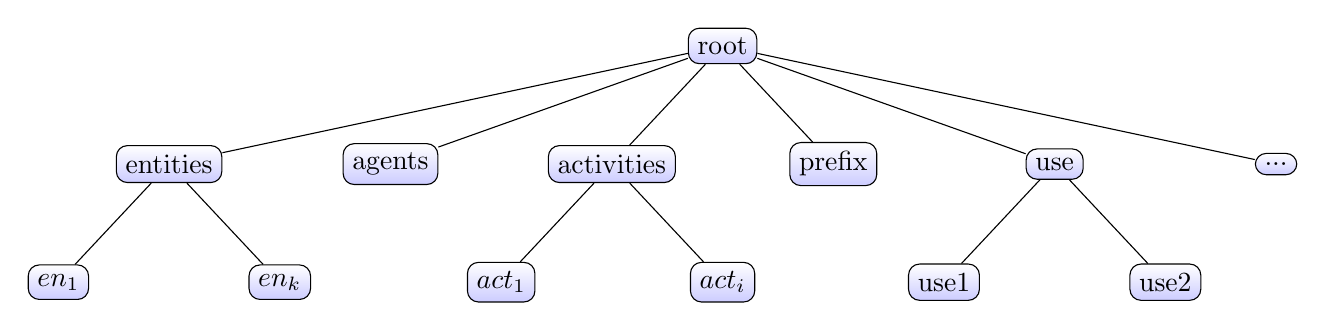
\begin{tikzpicture}[sibling distance=8em,
  every node/.style = {shape=rectangle, rounded corners,
    draw, align=center,
    top color=white, bottom color=blue!20}]]
  \node {root}
    child { node {entities}
         child { node {$en_1$} }
         child { node {$en_k$} }
     }
      child { node {agents} }
    child { node {activities}
      child { node {$act_1$} }
        child { node {$act_i$} }
        }
        child { node {prefix} }
        child { node {use}
        child { node {use1} }
        child { node {use2} }
        }
           child { node {...} }
        ;
\end{tikzpicture}
}
\end{center}
\end{minipage}
\caption{Top-key level of a PROV-JSON trace}
\label{prov-json-skeleton}
\end{figure}



The provenance traces represented in PROV-JSON format generally form a graph, that we define as follows. 

\begin{definition}[Provenance graph]
\label{def:prov-graph}
A provenance graph is a directed graph $G_P(V, R)$, where $V$ is the set of vertices and $R$ maps to provenance relationships.
Let $root \subseteq V$ be a set of vertices with an in-degree of 0 and an out-degree larger than 0. These nodes represent entities that are derived as described by the provenance trace. Successors of $root$ are entities $En \subseteq V$, activities $Act \subseteq V$, and agents $Ag \subseteq V$ involved in generating the entities described by $root$.
Each edge $e = (\langle v_{1},v_{2} \rangle,t)$, represents a provenance relation $r \subseteq R$ of type $t$ (e.g. gen, use) between $v_{1}$ and $v_{2}$  where   $\{v_{1},v_{2}\} \subseteq V$.
\end{definition}


    Figure~\ref{fig:universityX} depicts an example of a provenance graph.
     %obtained  {\color{Fuchsia} when exploring data warehouses using \prototype{}, the instance of our visual data exploration framework \framework{}.
%    It describes the why-provenance of the result ranking of ``MIT'', that is, it returns the source data relevant to produce this result.
%    The set  $root$ contains a unique entity ``entity1'' that results from the ranking query.
%    This latter is presented as an activity that uses the entity ``entity0'' to generate the result. 
%    Figure~\ref{fig:universityX} further includes white boxes associated with each node in the provenance graph. These contain the concrete provenance information recorded for each node. For instance, the provenance recorded about ``entity1'' includes the name of the university and the ranking value.
    It describes the set of explorations steps (cf.~Definition~\ref{def:expo-step}, Page~\pageref{def:expo-step}) investigated  by the user. The set  $root$ contains the entity ``entity2'' (corresponding to the last reached exploration step )  and  the agent ``agent1'' (corresponding to the user). Figure~\ref{fig:universityX} further includes white boxes associated with each node in the provenance graph. These contain the concrete provenance information recorded for each node. For instance, the provenance recorded about ``entity2'' includes the ids of the query and the visualization inspected by the users.

\smallskip


\noindent \textbf{Structure-based provenance summarization. } The set of provenance graphs defined above serve as input to our structure-based provenance summary approach, which consists of two steps. First, we infer individual provenance structures associated to individual provenance traces (local structures inference in Figure~\ref{fig:overview}). The second step aggregates individual structures into a single W3C-PROV compliant graph that structurally summarizes input provenance traces. 
More formally, we define the structure-based summary graph as follows.


\begin{definition}[Structure-based summary graph]A structure-based summary graph is a W3C-PROV compliant directed graph $SSG(PS_s, RS_s)$ associated to a set of provenance graphs $G$=\{$G_{P1}, \ldots,G_{Pn}$\} where $PS_s$ is the set of vertices referring to provenance structures defined later in Definition~\ref{def:prov-type} and $RS_s$ are edges mapping to the set of inferred provenance relationships. %\mel{Re reviewer 1: maybe ref to inference rules?)} 
Each relation $r \subseteq RS_s$ is presented as $ (\langle ps_{1},ps_{2}\rangle,t,c)$ where  $\langle ps_{1},ps_{2}\rangle$ is the edge connecting two structures $ps_1, ps_2 \in PS_s$, the type $t$ presents the provenance relationship type, and the cardinality $c$ is the number of provenance relationships in $G$, that follow the structure of $r$.
%quantifies the coverage of $r$ in $G$. 
\end{definition}


Figure~\ref{fig:Inf-type-university} shows an example of a structure-based summary graph. % inferred using our approach from provenance traces discussed in our illustrative Example~\ref{par:example}.
The content of this graph is discussed in Example~\ref{par:example2}.





\noindent \textbf{Visualization and analysis.} %To support users for different kinds of analysis over the structure-based summary graph, the last component of our pipeline provides different visualizations thereof.
The last component of our pipeline generates visualizations suited for various visual analysis tasks that rely on the structure-based summary graph. 
%{\color{Fuchsia}In contrast to previous steps depicted in Figure~\ref{fig:overview} that implement the \emph{provenance engine} module of our framework \framework{},  the visualization and analysis step describes possible techniques that can be used to implement the \emph{data display} module present also in the architecture of our framework \framework{} (cf.~Figure~\ref{fig:archi-FW}).}



\smallskip
%After this overview of the individual components of our solution, we now delve into the details of the structure-based provenance summarization component (Figure~\ref{sec:system}) and the visualization component (Figure~\ref{sec:vis}).
After this overview, we now delve into the details of individual components of our solution in Section~\ref{sec:system} and Section~\ref{sec:vis}.




\section{Provenance structure inference}
\label{sec:system}
\begin{figure}[b]
\[  \scalemath{0.8}{
\begin{array}{lllllll}
p ::=  Act \mid En \mid Ag  & \text{provenance high level types} \\
Act,En,Ag ::=  \epsilon \mid R  & \text{provenance types} \\
R ::=	\{ l_1:s_1, \ldots, l_i:s_i \}    & \text{Record type} \\
s::=    R \mid A \mid Bs  & \text{structure types} \\
A ::=  [s_1, \ldots,s_j]&\text{Array type} \\
B ::=	 \nule \mid Bool \mid \ Num \  \mid \ Str  & \text{Basic type}\\
\end{array} }
\]
 \vspace{-1.5em}
\caption{Syntax of provenance types}
\label{fig:datamodel}
\end{figure}





Figure~\ref{prov-json-skeleton} shows the top-key level structure of a PROV-JSON provenance trace, which contains nodes referring to W3C-PROV relationships (e.g., use, gen). Those nodes have always standard structures respecting the constraints defined in the W3C-PROV data model. In contrast, nodes mapping to entities, activities, and agents may have various structures (e.g., entities ``entity0'' and ``entity1'' in Figure~\ref{fig:universityX}) depending  on the underlying provenance collector.
Hence, a special focus is given in what follows to the subset of top-key level's elements, called provenance components, that contains entities, activities, and agents.
The provenance components follow the syntax shown in Figure~\ref{fig:datamodel}, extending the syntax proposed in~\cite{baazizi2017} to fit the content of W3C-JSON provenance traces. 



A provenance component $p$ is either an activity ($Act$), entity ($En$) or agent ($Ag$) type. 
These provenance high level types encompass records that are sets of pairs. Each pair has a label $l_i$ associated with a structure type $s$.
This latter could be a record, an array, or a basic type.
The array type is a sequence of structure types $s$ while basic values $B$ comprise $null$ values, booleans $Bool$, numbers $Num$, and strings $Str$.





%\subsection{Prov-type inference}
\subsection{Provenance component type inference}
The first phase of our approach performs a type inference for each provenance component $p$ present in the provenance trace. We adjust the inference rules proposed in~\cite{baazizi2017} to infer types called in what follows \emph{prov-types} defined in Figure~\ref{fig:datamodel}.

Prov-type inference is done according to the inference rules in Figure~\ref{fig:typinf}.
We distinguish two types of inference rules: (i)~those without premise: they infer the prov-type of value by simply reflecting the type of the value itself and (ii)~rules with premise: they require the recursive prov-type inference of each element present in the premise to generate the global prov-type indicated in the conclusion part. 



 \begin{figure}[t]
 \centering
\scalemath{0.75}{
 \begin{tabular}{llll}
 \staterule{(\textsc{TypeEmpty})}
   {}
   {
	% \judbasee{\{ \} }{  \{\} }
	 \judbasee{\{ \} }{ \tnull }
	 }
 &
 \staterule{\small(\textsc{TypeBool})}
  {}
 {\judbasee{true/false}{\tbool}}
  \\ \\
 \staterule{(\textsc{TypeNumber})}
   {s \in Number}
   {\judbasee{s}{\tnum}}
 &
 \staterule{(\textsc{TypeString})}
   {s \in String}
   {\judbasee{s}{\tstr}}
\\ \\
 \multicolumn{1}{c}{\staterule{(\textsc{TypeArray})}
{\judbasee{s_1,\ldots s_n}{T_1,\ldots,T_n} }
{\judbasee{[s_1,\dots,s_n]}{[T_1,\dots,T_n]}} }
   &
 \multicolumn{2}{c}{\staterule{(\textsc{TypeRec})}
 {\judbasee{s_i}{T_i} \ \ \judbasee{s_j}{T_j} \ \ \forall \textsc{ }{i},{j} \textsc{ }  i\neq j \Rightarrow l_i \neq l_j
 }
 {
 \judbasee{\{\fieldd{l_1}{s_i}, \ldots, \fieldd{l_i}{s_i} \} }{ \{\fieldd{l_1}{T_i}, \ldots, \fieldd{l_i}{T_i} \} }
 }}
  \\ \\

      \multicolumn{1}{c}{\staterule{(\textsc{TypeAgent})}
 {\judbasee{s}{T} }
 {\judbasee{Ag(s)}{Agent(T)}} }
&
   \multicolumn{1}{c}{\staterule{(\textsc{TypeAct})}
 {\judbasee{s}{T} }
 {\judbasee{Act(s)}{Activity(T)}} }
   &
   \multicolumn{1}{c}{\staterule{(\textsc{TypeEntity})}
 {\judbasee{s}{T} }
 {\judbasee{En(s)}{Entity(T)}} }
 \end{tabular}
}
 \caption{\label{fig:typinf}Prov-type inference rules.}
 \end{figure}



Based on inference rules presented in Figure~\ref{fig:typinf}, we can define {\emph{prov-type}}, the first step towards generating a structural provenance summary of a collection of provenance traces.
\begin{definition}[Prov-type]
\label{def:prov-type}
A prov-type for a vertex $v$ present in $G_P(V, R)$ corresponds to the structure inferred for~$v$.
\end{definition}

\begin{example}[Example of inferred prov-types]
Following our definition, the prov-type inferred for the entity ``entity0'' shown in Figure~\ref{fig:universityX} is:
\begin{center}
\small
\begin{adjustbox}{width=0.4\columnwidth,center}
\begin{tabular}{l}
\{ ``Entity'': \\
\hspace{0.5cm}	\{ \\
\hspace{0.5cm}\hspace{0.5cm}	``exp:queryID'': Num, \\
\hspace{0.5cm}\hspace{0.5cm}	``exp:visID'': Num \\
\hspace{0.5cm}	\} \\
\}
\end{tabular}
\end{adjustbox}
\end{center}
This prov-type is inferred using the recursive \emph{TypeRec} inference rule depicted in Figure~\ref{fig:typinf}. This rule is recursive. Accordingly, we iterate over key-values pairs present in entity ``entity0'' shown in Figure~\ref{fig:universityX}. For each key-value pair, we maintain the key and we apply a basic inference rule on the value (see \emph{TypeNumber} rule depicted in Figure~\ref{fig:typinf}).  Finally, the set of key and their associated basic types are grouped and returned as a result of the recursive \emph{TypeRec} inference rule.

\end{example}

\subsection{Individual structural provenance graph}
Once we compute the prov-type of each vertex in a provenance graph, we are able to infer the individual structural provenance graph that we define as follows.
\begin{definition}[Individual structural provenance graph]
  \label{def:temp-prov}
$GS(P_s, R_s)$ is an individual structural provenance graph associated to a provenance graph $G_P(V, R)$.
It is a W3C-PROV compliant directed graph where $P_s$ is the set of prov-types for all $v \in V$ and $R_s$ is the set of inferred relationships structures: 
Each edge $e_s = (\langle ps_1, ps_2\rangle,t,c)$ is a provenance relationship structure in $R_s$ between two structures $\{ps_1, ps_2\} \subseteq P_s$. The edge $e_s$ is labeled by $t$ that refers to the type of provenance relationship and  by a cardinality $c$ computed as  $c=|R_{sim}|$ such that  $R_{sim}\subseteq R$ and  $\forall  e_r=(\langle v_1, v_2\rangle,t') \in R_{sim}$, $e_s.t=e_r.t'$ holds and  $\forall i  \in \{1,2\},  \exists j  \in \{1,2\}$ such that the prov-type of $v_{i}$ is equal to $ps_j$. 
\end{definition}


Note that the following properties hold for the individual structural provenance graph $GS(P_s, R_s)$:

\begin{lemma}[Properties of structural provenance graph]
\label{def:prop}
For a structural provenance graph $GS(P_s, R_s)$, we have
\begin{itemize}
\item  $\forall ps ,ps'  \in P_s$,   $ps \neq ps'$
\item  $\forall p_s  \in P_s  $, $  \exists$  $v \in V$  such that its prov-type is equal to $p_s$
\item  $\forall e_s=(\langle ps_1, ps_2\rangle,t,c) \in R_s, \exists e=(\langle v_1, v_2\rangle,t') \in R$  such that $e_s.t=e.t'$ and $ \forall i  \in \{1,2\}, \exists j  \in \{1,2\} $ such that the prov-type of $v_{i}$ is equal to $ps_j$.
\end{itemize}
\end{lemma}

\begin{figure}[t]
\centering
\includegraphics[scale=0.4]{figures/Tapp19/EvoPROV_provSummary}
\caption{Structural summary of MIT's ranking provenance}
\label{scheme:universityX}
\end{figure}
Figure~\ref{scheme:universityX} shows an example of individual structural provenance graph associated to the excerpt of W3C-PROV evolution provenance graph shown in Figure~\ref{fig:universityX}.  It contains 6 nodes whose prov-types are shown in white boxes below each vertex. For instance, the node ``actSt0'' has a prov-type that was inferred from the node ``Activity0'' present in Figure~\ref{fig:universityX}. 
Figure~\ref{scheme:universityX} depicts also cardinalities and types associated with each edge.
For instance, the edge between ``actSt1'' and ``agSt0'' has the type ``association'' and a cardinality equals to one.
The cardinality is explained by the provenance graph shown in Figure~\ref{fig:universityX} where we have one edge of type ``association'' between nodes ``activity1'' and ``agent1''.




To infer an individual structural provenance graph, we leverage the following two fundamental definitions.
\begin{definition}[Vertex structural equality]
    \label{lm:vert}
Given a provenance graph $G_P(V, R)$, we say that two vertices are structurally equal if they have the same prov-type.
\end{definition}
\begin{definition}[Edge structural equality]
  \label{lm:edge} 
We consider that edges $(\langle el1_{1},el1_{2}\rangle,t_{1})$ and $(\langle el2_{1},el2_{2}\rangle,t_{2})$ are structurally equal if they have the same provenance relationship type ($t_1=t_2$),  
%and $ \forall i  \in \{1,2\}, \exists j  \in \{1,2\} $ such that $el1_i$ and $el2_j$  are structurally equal.
vertices $el1_1$ and $el2_1$  are structurally equal,  and vertices $el1_2$ and $el2_2$  are structurally equal.
%($el1_1$ , $el2_1$)  and  ($el1_2$ , $el2_2$)  are structurally equal.
\end{definition}


\begin{algorithm}[t]
%\scriptsize
\caption{Individual Prov Structure Inf ($G_p$)}
\label{algo:IndividualSchemaInf}
 \KwIn{$G_p$ : provenance graph}
  \KwOut{$GS$: individual structural provenance graph}
    $s_{cand} \leftarrow $  an empty map of $\langle S, id \rangle$ elements,  where $S$ is the prov-type, and  $id$ is an identifier of a provenance component\;
  $ST_{inf} \leftarrow $ an empty hash-map of $\langle S,L(id) \rangle$ elements,  where $S$ is the prov-type, and  $L(id)$ is the list of provenance components ids following $S$\;
  $REL_{Inf} \leftarrow $ an initially empty list of $\langle \{d_1..d_k\},t,c \rangle$ elements,  where $t$ refers to the type of provenance relation, $\{d_1..d_k\}$ are related provenance components and $c$ refers to the cardinality  \;

{\tcc{Inference of provenance components structures}}
		%\ForEach{$e \in G_p.Entity() \cup  G_p.Activity() \cup G_p.Agent() $
		\ForEach{$e \in G_p.getVertices()$} {   \label{algoInfType:line4}
 	  			  $S_{cand} \leftarrow  Add( \langle InferType(e),e.getId()  \rangle )$\; \label{algoInfType:line5}
		}
	{\tcc{Aggregation of prov-types}}	
	$ST_{inf} \leftarrow  AggregateTypes(S_{cand})$\;	 \label{algoInfType:line6}
	{\tcc{Inference of provenance relations structures}}

	\ForEach{$r \in G_p.getRelations() $}{   \label{algoInfType:line7}
 
        $r_{rel} \leftarrow r.getRelationsElements()$\;
        $s_{rel} \leftarrow \emptyset $ \;
          \ForEach{$comp \in r_{rel} $}{
           $ s_{rel} \leftarrow  Add (ST_{Inf}.get(comp.getID())  )  $\;
          }
             $REL_{Inf} \leftarrow  Add( s_{rel},r.getType,1)$\;  \label{algoInfType:line12}
           }
{\tcc{Provenance relations structures aggregation}}
$REL_{Inf} \leftarrow  AggregateRels(REL_{inf})$\;  \label{algoInfType:line13}
$ GS  \leftarrow $ new Graph $ (ST_{inf},REL_{inf}) $\; 
return $GS$\;

\end{algorithm}


Algorithm~\ref{algo:IndividualSchemaInf} leverages the two previous definitions to infer an individual structural provenance graph for a provenance graph $G_p$.
Firstly, we go over the provenance components (lines~\ref{algoInfType:line4}--\ref{algoInfType:line5}) and we generate their associated prov-types using the function $InferType$ that implements the rules specified in Figure~\ref{fig:typinf}.
Pairs of inferred structures and ids of provenance components are then stored in the map $s_{cand}$.
In line~\ref{algoInfType:line6}, we aggregate similar structures present in $s_{cand}$ based on Definition~\ref{lm:vert} and we store results in $ST_{inf}$ that contains inferred prov-type $s$ and the full ids list of provenance components that follow $s$. 

Afterwards, we go over provenance relationships~(lines ~\ref{algoInfType:line7}--~\ref{algoInfType:line12}). 
Recall that a provenance relationship specified in Definition~\ref{def:prov-graph} is an edge between two provenance components.
Hence, we identify for each relationship $r$, ids of provenance components involved in $r$. We resort to the $ST_{inf}$ to replace the set of ids by their corresponding prov-types. 
Later, we store identified prov-types, the type of $r$, and a cardinality (set to one) in $REL_{inf}$ (line~\ref{algoInfType:line12}). 
Finally, we aggregate in line~\ref{algoInfType:line13} the cardinality of relationships that are structurally equal using function $AggregateRels$ that implements Definition~\ref{lm:edge}.

Once we specify the set of prov-types $ST_{inf}$ and the set of inferred relationships $REL_{inf}$, 
our Algorithm~\ref{algo:IndividualSchemaInf} returns $GS$, the individual structural provenance graph of $G_p$.
%\mel{make index on ids rather on structure} \hou{we are dealing with several provenance graphs, the same id can be present in many provenance traces}





\subsection{Structure-based summary graph generation}
At this stage, our goal is to further aggregate the set of individual structural provenance graphs returned by the previous step in order to generate a unique structure-based summary.  We choose to apply an exact merge to fuse input structural summary graphs. 
For that, we leverage again Definition~\ref{lm:vert} and Definition~\ref{lm:edge} to merge  vertices and edges of individual structural graphs that are structurally equal. 


Our choice of exact merge is justified by its capability to mitigate the loss of information by providing exact structures available in a set of provenance traces. 
This is not the case for the inexact merge that fuses nodes having different yet compatible structures.
While our approach could be extended to support the inexact merge, we prefer to leave it for future research to assess or convey the impact of inexact merge techniques on visual analytics tasks. 
Based on the current implementation of merge,  we can redefine the structure-based summary graph as follows.



\begin{lemma}[Structure-based summary graph properties] 
\label{prop:sum-graph}
The structure-based summary graph $SSG(PS_s, RS_s)=  \bigcup_{i=1}^n  GS_i(P_{si}, R_{si})$ where $GS_i$ are individual structural provenance graphs.
It has a surjective map $M$: $ \bigcup_{i=1}^n P_{si} \longrightarrow PS_s$ such that:\begin{itemize}[noitemsep]
\item  $\forall p\in P_{si}, \exists p^*\in PS_s$ with $p$ and $p^*$ are structurally equal
\item  $\forall r \in R_{si},  \exists$ $r^* \in RS_s$ with $r$ and $r^*$ are structurally equal
\end{itemize}
\end{lemma}
%\mel{Maybe add that it is straightforward to define an iterative approach to merge graphs, which we thus do not further discuss here. The map reduce part would I think better fit in the implementation section (I still do not find the map reduce relevant / helpful though).}
While it is possible to incrementally perform a set of pairwise merges of individual structural provenance graphs to construct the structure-based summary graph, we choose to design the structure-based summary inference using a map-reduce model to ensure the capability of processing large collections of provenance traces. 
We justify our choice of this model by the soundness property already proved for the structure inference approach~\cite{baazizi2017}. Our approach enjoys also commutativity and associativity properties as we use an exact matching strategy to aggregate structures.  These are important properties since the map-reduce model may arbitrarily split the input set of provenance traces.
We postpone the discussion of the performance study of our approach to the Section~\ref{sec:casestudy}.





\section{Visual analysis of summary graphs}
\label{sec:vis}
Based on the structure-based summary graph for a collection of provenance traces obtained as described in the previous section, we define several visual analysis tasks that apply to this kind of summary. For each task, we also evoke visualization techniques/interactions that potentially fit the task. 
%{\color{Fuchsia}Based on the structure-based summary graph output using the instance of our framework \framework{}, we define several visual exploration tasks that apply on this kind of summary. For each task, we also evoke visualization techniques that potentially fit the task and that can be implemented in the \emph{data display} sub-module present in the architecture of our framework \framework{} (cf.~\ref{fig:archi-FW}). }


\begin{enumerate}
%\vspace{-1em}
\item \emph{High level overview }
The primary goal of our approach is to generate a structural summary that is  easy to read and that allows analysts to easily grasp which different structures are present in the provenance traces. To avoid overwhelming analysts with too many details at an early stage of their analysis, the visualization should be limited to the rendering of basic information such as vertices and edges representative of structures and provenance relationships. \label{itm:t1}   


\item \emph{Interactive visual analysis }  Rendering a simple visualization of structure-based summary facilitates the analysis task. 
Further information can be offered on demand using interaction, e.g., hovering over nodes or edges. \label{itm:t2} 



\item \emph{Visual comparison } Possible visual analysis tasks include the comparison between the summary and provenance instances.
Here, an analyst may compare a particular provenance trace to the inferred structural summary graph. Brushing and linking interaction techniques could be employed in this task to render/highlight structures and their corresponding provenance traces. \label{itm:t3} 

\item \emph{Homogeneity overview } Our approach assigns cardinalities to edges present in the provenance structural summary graph.
This information should be communicated clearly as it serves to investigate the homogeneity/heterogeneity of analyzed provenance traces. Sankey diagrams~\cite{Riehmann:2015} are a candidate visualization for this task, given their ability to render edges with various width expressing the importance of cardinalities.
%We can also resort to the change of color encodings to highlight ``outliers'', e.g., in Example~\ref{par:example} where some edges have low cardinalities in comparison to the remaining edges in the summary graph. 


\item \emph{Visual identification of patterns }  Using cardinality information, we can reveal recurrent patterns among the set of analyzed provenance traces. The visualization should highlight sub-graphs having high cardinalities  compared to other information present in the summary graph. Sankey diagram~\cite{Riehmann:2015} could be used also for this analysis task. \label{itm:t5} 

\item \emph{Visualization of dense regions of the summary } Structure-based summary graphs may contain dense regions where vertices are highly connected.
This specific range of nodes may be subject of bottleneck or may present a heavily shared component.
Note that the presence of high connectivity can easily lead  to a cluttered visualization. 
To avoid that, we can use force-directed graphs that reduce edge crossings by making edges repel each other. \label{itm:t6} 



\end{enumerate}
The list of proposed visual analysis tasks and their visualizations is not exhaustive. Indeed, a thorough investigation of other possible visual analysis tasks is left for future research.
%{\color{Fuchsia}The list of proposed visual exploration tasks and their visualizations is not exhaustive. Indeed, a thorough investigation of other possible visual exploration tasks that can be made using this instance of our framework \framework{} is left for future research.}


\section{Case study}
\label{sec:casestudy}

We have shown initially in Examples~\ref{par:example} and~\ref{par:example2} that our structure-based summary graph facilitates the task of understanding users' behaviour when exploring visually data using our system \prototype{}.
In this section, we broaden the discussion to show the feasibility of our instance when exploring visually other types of provenance.
Alongside the description of these scenarios, we illustrate the feasibility of some visual exploration tasks discussed in Section~\ref{sec:vis}.  
%Note that, we provide a set of structure-based summary graph visualizations associated to the discussed scenarios that are available online~\cite{usecase:url}. 
%\hou{the link is not anymore available}


\subsubsection{Visual debugging of a tracked process}

Assume that our goal is to define a university ranking that consolidates three well-known university rankings\footnote{\url{https://www.kaggle.com/mylesoneill/world-university-rankings}}. As the different source rankings use different criteria, the three source tables do not fully agree. Hence, consolidation requires the definition of a custom score derived from the three sources. Now, let us assume that the custom score yields some surprising results, e.g., the university ``MIT''  is ranked at tenth position. To better understand the working of the ranking, we compute the why-provenance of the suspicious result, as shown in Figure~\ref{fig:universityX1}.
This trace alone is not very insightful yet. To this end, we compute the structure-based summary graph that  includes traces for all results (we limit to 10 results in our example). 


Our structure-based summary graph, shown in Figure~\ref{fig:Inf-type-university1} %(and available online~\cite{usecase:url}) 
summarizes the ten why-provenance traces associated with the top-ten query results. 
\begin{figure}[t]
\center
\includegraphics[scale= 0.4]{figures/Tapp19/example_traceMIT1.pdf}
\caption{Provenance for MIT custom rank}
\label{fig:universityX1}
\end{figure}
\begin{figure}[t]
\center
\includegraphics[scale= 0.35]{figures/Tapp19/example_trace_summary1.pdf}
\caption{Structural summary of ten provenance traces}
\label{fig:Inf-type-university1}
\end{figure}

From this graph, we see (Task \mycircle{\scriptsize A}) that while most results (all conforming to the structure ``entitySt1'') are derived from entities conforming to the structure of ``entitySt2'', one entity is derived from a different structure, i.e., ``entitySt0''(Task \mycircle{\scriptsize D}). Interaction with this summary graph allows us to identify ``entitySt0'' as the structure of the unexpected ``MIT'' result. Hence, this summary shows that ``activity1'' computing the consolidated ranking may be affected by an incomplete input table (i.e., no score from the third source is available).



Indeed, it turns out that the use of a full outer join in our ranking query is unreliable as it tolerates the integration of incomplete information. Specifically, MIT university has a different name in one of the three ranking tables. 
This entails the presence of a tuple resulting from joining two ranking tables, used later to compute the final score of MIT university. 





\subsubsection{Data integration flow transparency}

Our second use case considers a data integration process specified using the high-level integration language (HIL)~\cite{hernandez:edbt13}  incorporated in IBM Infosphere Master Data Management\footnote{\url{https://www.ibm.com/support/knowledgecenter/SSWSR9_11.4.0/com.ibm.swg.im.mdmhs.pmebi.doc/topics/using_hil.html}}.
The sample integration flow extracts information about key people of the US financial sector. It takes a set of reports generated by companies to construct a set of individual reports about persons' careers.
HIL was recently instrumented to capture provenance~\cite{Oppold:IPAW18}, allowing us to generate five provenance traces tracking the discussed flow when integrating information about five persons.
%These traces are converted subsequently to PROV-JSON format and they are summarized using our approach.
These traces are converted subsequently to PROV-JSON format. 

Assume now that we are interested in understanding and learning recurrent patterns in the discussed sample integration flow. Accordingly, we can compare visually the five generated provenance graphs.
Yet, this process is tedious given the wealth of content of processed provenance traces.
To this end, we resort to our structure-based summary approach that can facilitate the task of understanding  the tracked data integration process.

 

As shown in Figure~\ref{fig:IBM}, we render the summary output by our approach using a force-directed graph (Task \mycircle{\scriptsize A}) given its capacity to place in convenient way vertices and edges by assigning forces to them.



\begin{figure}[t]
 \includegraphics[scale=0.4]{figures/tapp19/HIL_annotated2.pdf}
 \caption{Structural summary for HIL provenance graphs}
 \label{fig:IBM}
\end{figure}
The inspection of Figure~\ref{fig:IBM} reveals two important pieces of information. Firstly, we observe that the structure highlighted using an orange dashed box corresponds to the outcome of the implemented data integration flow as it is the only structure having only relationships of type ``generation'' with three activities structures. This reveals also that this particular structure was populated by three integration sub-flows (Task \mycircle{\scriptsize E}). By tracing back interactively these sub-flows, we can learn more about the implemented data integration flow.


Furthermore, Figure~\ref{fig:IBM} shows a second important finding. Indeed, all data integration sub-processes stem from the single structure highlighted by a green dashed box (Task \mycircle{\scriptsize F}). This later presents the structure of input reports used by the tracked data integration process. 
By hovering over the interactive visualization of Figure~\ref{fig:IBM}, 
%(available online~\cite{usecase:url}), 
we can learn the structure of input reports.
For instance, the input reports contain personal information about the key people including their address, their positions, as well as information related to the reports such as the issuer (the editor) of a report and the ID of the issuer.






\subsubsection{Corroboration}
Our final use case comes from the life science domain relating to Next Generation Sequencing (NGS) and is inspired by~\cite{alawini:18}. 
This project presents a workflow including six possible analysis stages that are invoked differently depending on the version of the workflow. 
One major problem already mentioned in~\cite{alawini:18} is the lack of NGS workflow transparency. Tackling this problem resulted in the collection of more than 800 provenance traces, which are publicly available\footnote{\url{https://github.com/alawinia/provClustering/}}. 

\begin{table}[t]
\centering
\scriptsize
\sffamily\footnotesize
\tabulinesep=2pt
 \begin{tabu}{|p{1.5cm}|p{8cm}|} \hline 
pattern & clause  \\\hline
claim & wasGeneratedBy$(e_1, a_1)$ with \newline $e_1= $\{"foaf:name":\{"\$":"file.txt", "type":"string"\},"prov:type":\{"\$": "kimlab","type":"qualified\_name" \}\},\newline $a_1:\{$"kimlab:htseq-stranded": \{"\$": "gencode2","type":"string"\}\} \\\hline
confirmation pattern & wasGeneratedBy$(e_1, a_1)$ with \newline  $e_1= \{$"foaf:name": \{"\$": *,"type":*\}, "prov:type":\{"\$": *,"type":* $\}\},\newline a_1=\{$"kimlab:htseq-stranded":\{"\$": *,"type":*\}$\}$ \\\hline
witness pattern & wasGeneratedBy$(e_1, a_1)$ with \newline $e_1=\{*\}, a_1=\{*\}$ \\\hline
\end{tabu}
\caption{Clauses used in the corroboration process}
\label{tab:rw}
\end{table}


We assume that an analyst is working on this collection to study impacts of analysis stages on the generated results.
 Given the large size of this collection, the analyst randomly picks some provenance traces. The analysis of these traces reveals the presence of common information presented in the first row of Table~\ref{tab:rw}.  This clause states that an analysis stage called ``HTSeq'' presented as an activity $a_1$ is always involved in the generation of some intermediate results. As it is tedious to check all provenance traces, \emph{the analyst claims that data input to the tracked workflow is necessarily processed by the analysis stage ``HTSeq''}.

To assess the truthfulness of the analyst's claim, we resort to the approach proposed in~\cite{Barakat:17}. 
It extracts the set of confirmation patterns (witnesses confirming the structure of the claim) and the set of witness patterns (generic version of the claim) from the existing provenance traces. The second and third rows of Table~\ref{tab:rw} describe these two sets, which are finally compared to compute the reliability of the claim. 

%Note that clauses of confirmation and witness patterns could be easily inferred using our approach. Hence, we generate the structure-based summary graph representative of provenance traces available in the analyzed repository.
Note that clauses of confirmation and witness patterns can be easily inferred using our approach. Hence, we use our approach to summarize provenance traces available in this provenance repository.



Figure~\ref{fig:corroboration} depicts an excerpt of the structure-based summary graph. We choose to only render  the set of structural relationships of type ``generation'' since they map to the witnesses set specified in the third row of Table~\ref{tab:rw} (Task \mycircle{\scriptsize E}). For that, we use a Sankey diagram as we need to highlight the cardinality of inferred relationships' structures that will be used to estimate the reliability of the claim.
\begin{figure}[t]
 \includegraphics[scale=0.4]{figures/tapp19/alawini_annotated.pdf}
 \caption{Excerpt of structural provenance summary graph}
 \label{fig:corroboration}
\end{figure}
Indeed, the width of edges in the Sankey diagram corresponds to the cardinality value of inferred relationships.
For instance, we can easily find the set of confirmation patterns (confirming the second row of Table~\ref{tab:rw}) which corresponds to the edge between nodes ``ActSt5'' and ``EntSt1''. The cardinality of this relationship is not high given the mediocre width of this particular edge. Based on this visualization, 
%(available in~\cite{usecase:url}), 
we can get a rough idea about the reliability of the claim (Task \mycircle{\scriptsize D}) which seems not high as the number of confirming patterns is significantly less than the number of witnesses (sum of all edges).
We can also learn interactively structures and exact cardinalities, that are used to compute the exact value of the reliability of the claim following formulas proposed in~\cite{Barakat:17}.


%\mel{This use case is not easily understandable when not already familiar with it. Maybe write from the perspective of a scientist? What are the questions they want to answer, e.g., is my claim correct, what frequent patterns exist? Then show how the structural summary helps to answer these questions.\\For all use cases, can you revisit why existing approaches are not useful for the type of analyis? This would then somehow serve as a qualitative evaluation (compared to existing approaches).}




%\section{Performance evaluation}
\section{Evaluation of the structure-based provenance summary approach}
\label{sec:evaluation}
{%\color{Fuchsia}
While the previous section focused on presenting the use cases that illustrate the usefulness of our structure-based provenance summary, this section evaluates our approach qualitatively.
More specifically, we evaluate in this section the performance of our structure-based provenance summary in terms of conciseness and runtime.
To this end, we use in this experiment provenance traces of use cases $UC1$, $UC2$, and $UC3$, referring to the three case studies discussed in Section~\ref{sec:casestudy}.
We implement also two types of provenance generators: (i)~the first generator $gen_{prov}$ generates many provenance traces according to the structure of a real provenance traces, (ii)~$gen_{struct_{prov}}$:  generates  provenance traces having new structures derived from the structures available in the seed provenance traces. It introduces random changes to the structure of each seed. The new structures are used to generated synthetic provenance traces.



 \begin{table}[b]
\centering
\scriptsize
 \begin{tabu}{|p{1.5cm}|p{2.5cm}|p{2.5cm}|p{2.5cm}|} \hline
Use case & avg(\#activities) & avg(\#entities) & avg(\#relations)\\ \hline
 $UC1$&1&11.4& 21.8  \\ 
  $UC2$&114.2&115.3& 228.6  \\ 
   $UC3$&5&6& 23  \\ 
 \hline
\end{tabu}
\caption{Overview of processed provenance traces}
\label{tab:prov-stats}
\end{table}
We have studied firstly the conciseness of summary graphs output by our structure-based provenance summary approach.
%{\color{Fuchsia}
This metric is computed as the ratio of the number of inferred structures (of type entity, activity, and relations) to the total number of entities, activities, and relations in the input provenance traces set.%}
As mentioned previously, we considered provenance traces of use cases $UC1$, $UC2$, and $UC3$, referring to the three case studies discussed in Section~\ref{sec:casestudy}. 
For each use case, we collect ten provenance traces whose graphs information are summarized in Table~\ref{tab:prov-stats}.
We generate for each provenance set ($UC1$, $UC2$, and $UC3$), its structure-based summary graph. Accordingly, we compute the conciseness rate by comparing the number of inferred structures (of type entity, activity, and relations) with the number of entities, activities, and relations in the input provenance traces set.
As shown in Figure~\ref{fig:exper1}, our approach performs a high simplification rate above 80\%) for the three studied use cases. This indicates that structure-based summary graphs allow producing concise summaries of collections of provenance traces.


\begin{figure}[t]
  \centering
  \includegraphics[scale=0.37]{figures/tapp19/simplification_rate.pdf}
  \caption{Conciseness rate for diverse case studies}
  \label{fig:exper1}
\end{figure}

 So far, we have studied the conciseness of our structures-based summary graph when processing provenance sets that are highly homogenous (i.e., processed provenance traces in each set have roughly the same structure). Yet, this conciseness rate may be impacted by the degree of heterogeneity of processed set of provenance traces. 
To this end, we study in the following experiment the impact of heterogeneity degree (i.e, the inconsistency rate of structures of processed provenance traces) on the conciseness of inferred provenance summaries. 
%{\color{Fuchsia}Note that we consider that two provenance traces are heterogeneous if their corresponding structures are inconsistent e.i., . }
To do that, we use first our provenance generator  $gen_{struct_{prov}}$ (described above) to prepare four provenance traces set containing consecutively 10, 25, 50, and 100 provenance traces with different structures. Later, these provenance sets are increased using our provenance generator $gen_{prov}$ (described above) until they reach the size of 200 provenance traces. Ultimately, we have four provenance traces sets, each containing 200 provenance traces but with various degree of heterogeneity (5\%, 12.5\%, 25\% and 50\%).
Note that the degree of heterogeneity is computed as the set of different structures available in a provenance set divided by the size of the provenance set.
For instance, to get a heterogeneity degree equal to 5\%, our generator $gen_{struct_{prov}}$ outputs 10 provenance traces with 10 different structures. These structures are used by $gen_{prov}$to generate 200 provenance traces.

At this stage, we employ our structures-based summary approach to process provenance traces. Later, we measure the conciseness of our approach by comparing the number of inferred structures (of type agent, entity, activity, and relations) with the number of agents, entities, activities, and relations in each input provenance traces set.
For each processed set of provenance traces, we compute the reduction rate that corresponds to the comparison between the size of the output summary graph's size with the size of provenance traces present in the processed set ($\frac{size\_summary\_graph }{\sum size\_processed\_provenance\_traces}$).

\begin{figure}[t]
  \centering
 \includegraphics[scale=0.65]{figures/tapp19/heterogeneity.pdf}
  \caption{Impact of  input provenance heterogeneity on the structural provenance summary conciseness}
     \label{fig:hetero}
\end{figure}

Figure~\ref{fig:hetero} depicts the impact of heterogeneity degree on the conciseness of the inferred structure-summary graph. 
As expected, the heterogeneity of provenance traces impacts the conciseness. Indeed, the conciseness rate decreases as the heterogeneity between processed provenance traces increases. Yet, we see that our structure-based summary approach maintains an acceptable rate of conciseness even for highly heterogeneous provenance traces sets (e.g., when heterogeneity rate= \%50).


We have also studied the runtime of our approach implemented using a map-reduce model.
Accordingly, we generate using $gen_{prov}$ several synthetic provenance traces based on real provenance traces available in $UC1$, $UC2$, and $UC3$.
This results in several synthetic provenance trace sets of varying sizes, that are summarized later using our approach. We performed our experiments on a cluster containing 3 nodes, each containing 6 cores and 256GB of RAM.
During experiments, we measured runtimes of the two main steps of our approach (shown in Figure~\ref{fig:overview}): (i)~$LocalInf$ maps to the local inference of structures and (ii)~$GlobalAgg$ concerns the aggregation of structures.
 Figure~\ref{fig:exper22} reports the runtimes of the two steps on a logarithmic scale over various sizes of provenance trace collections.
 The two steps have initially similar runtimes when processing small provenance traces sets. Yet, the gap between the two steps increases clearly with the number of processed provenance traces.  
 Indeed, as the number of provenance traces increases, the size of the hash map storing inferred structures and their associated objects increases. 
Later, hash map values storing large lists, are accessed during the global aggregation to group edges that are structurally equal. This is costly and leads to an increase of global aggregation runtime.

\begin{figure}[t]
  \centering
  \includegraphics[scale=0.5]{figures/tapp19/runtime.pdf}
  \caption{Runtime of summary computation steps}
    \label{fig:exper22}
\end{figure}



\section{Summary and future work}
In this chapter, we present our approach that infers a structure-based summary from a set of provenance traces available in PROV-JSON format.
We discuss our proposed solution as well as possible visual analytics tasks that may be applied to this type of summary. 
We show how our approach can contribute to the analysis of a set of evolution provenance graphs generated using our visual data exploration framework \framework{}. Furthermore, we broaden the discussion of the utility of our approach by providing other illustrative use cases treating other types of provenance.
%We implement also our approach using a map-reduce fashion. 
Our preliminary experimental evaluation studies both the runtime and conciseness of summarization. Several points for future research have been mentioned throughout this work, including the integration of schema inference and schema integration techniques to our approach as well as a thorough study and evaluation of different visualizations for different analytical tasks.



